%step through each section of the atlas detector
%could spend more time on the muon spectrometer (like the new EE A-side detectors)
%and more time on the muon trigger
%Clare put in the minimal detail (no more than 20 pages) while Jeremy had 50 pages
%I could maybe fit somewhere in between

%need to define Muon Spectrometer (MS)
%need to define Inner Detector (ID)
%Assumptions:
%Will describe trigger

\begin{figure}[ht!]
\centering
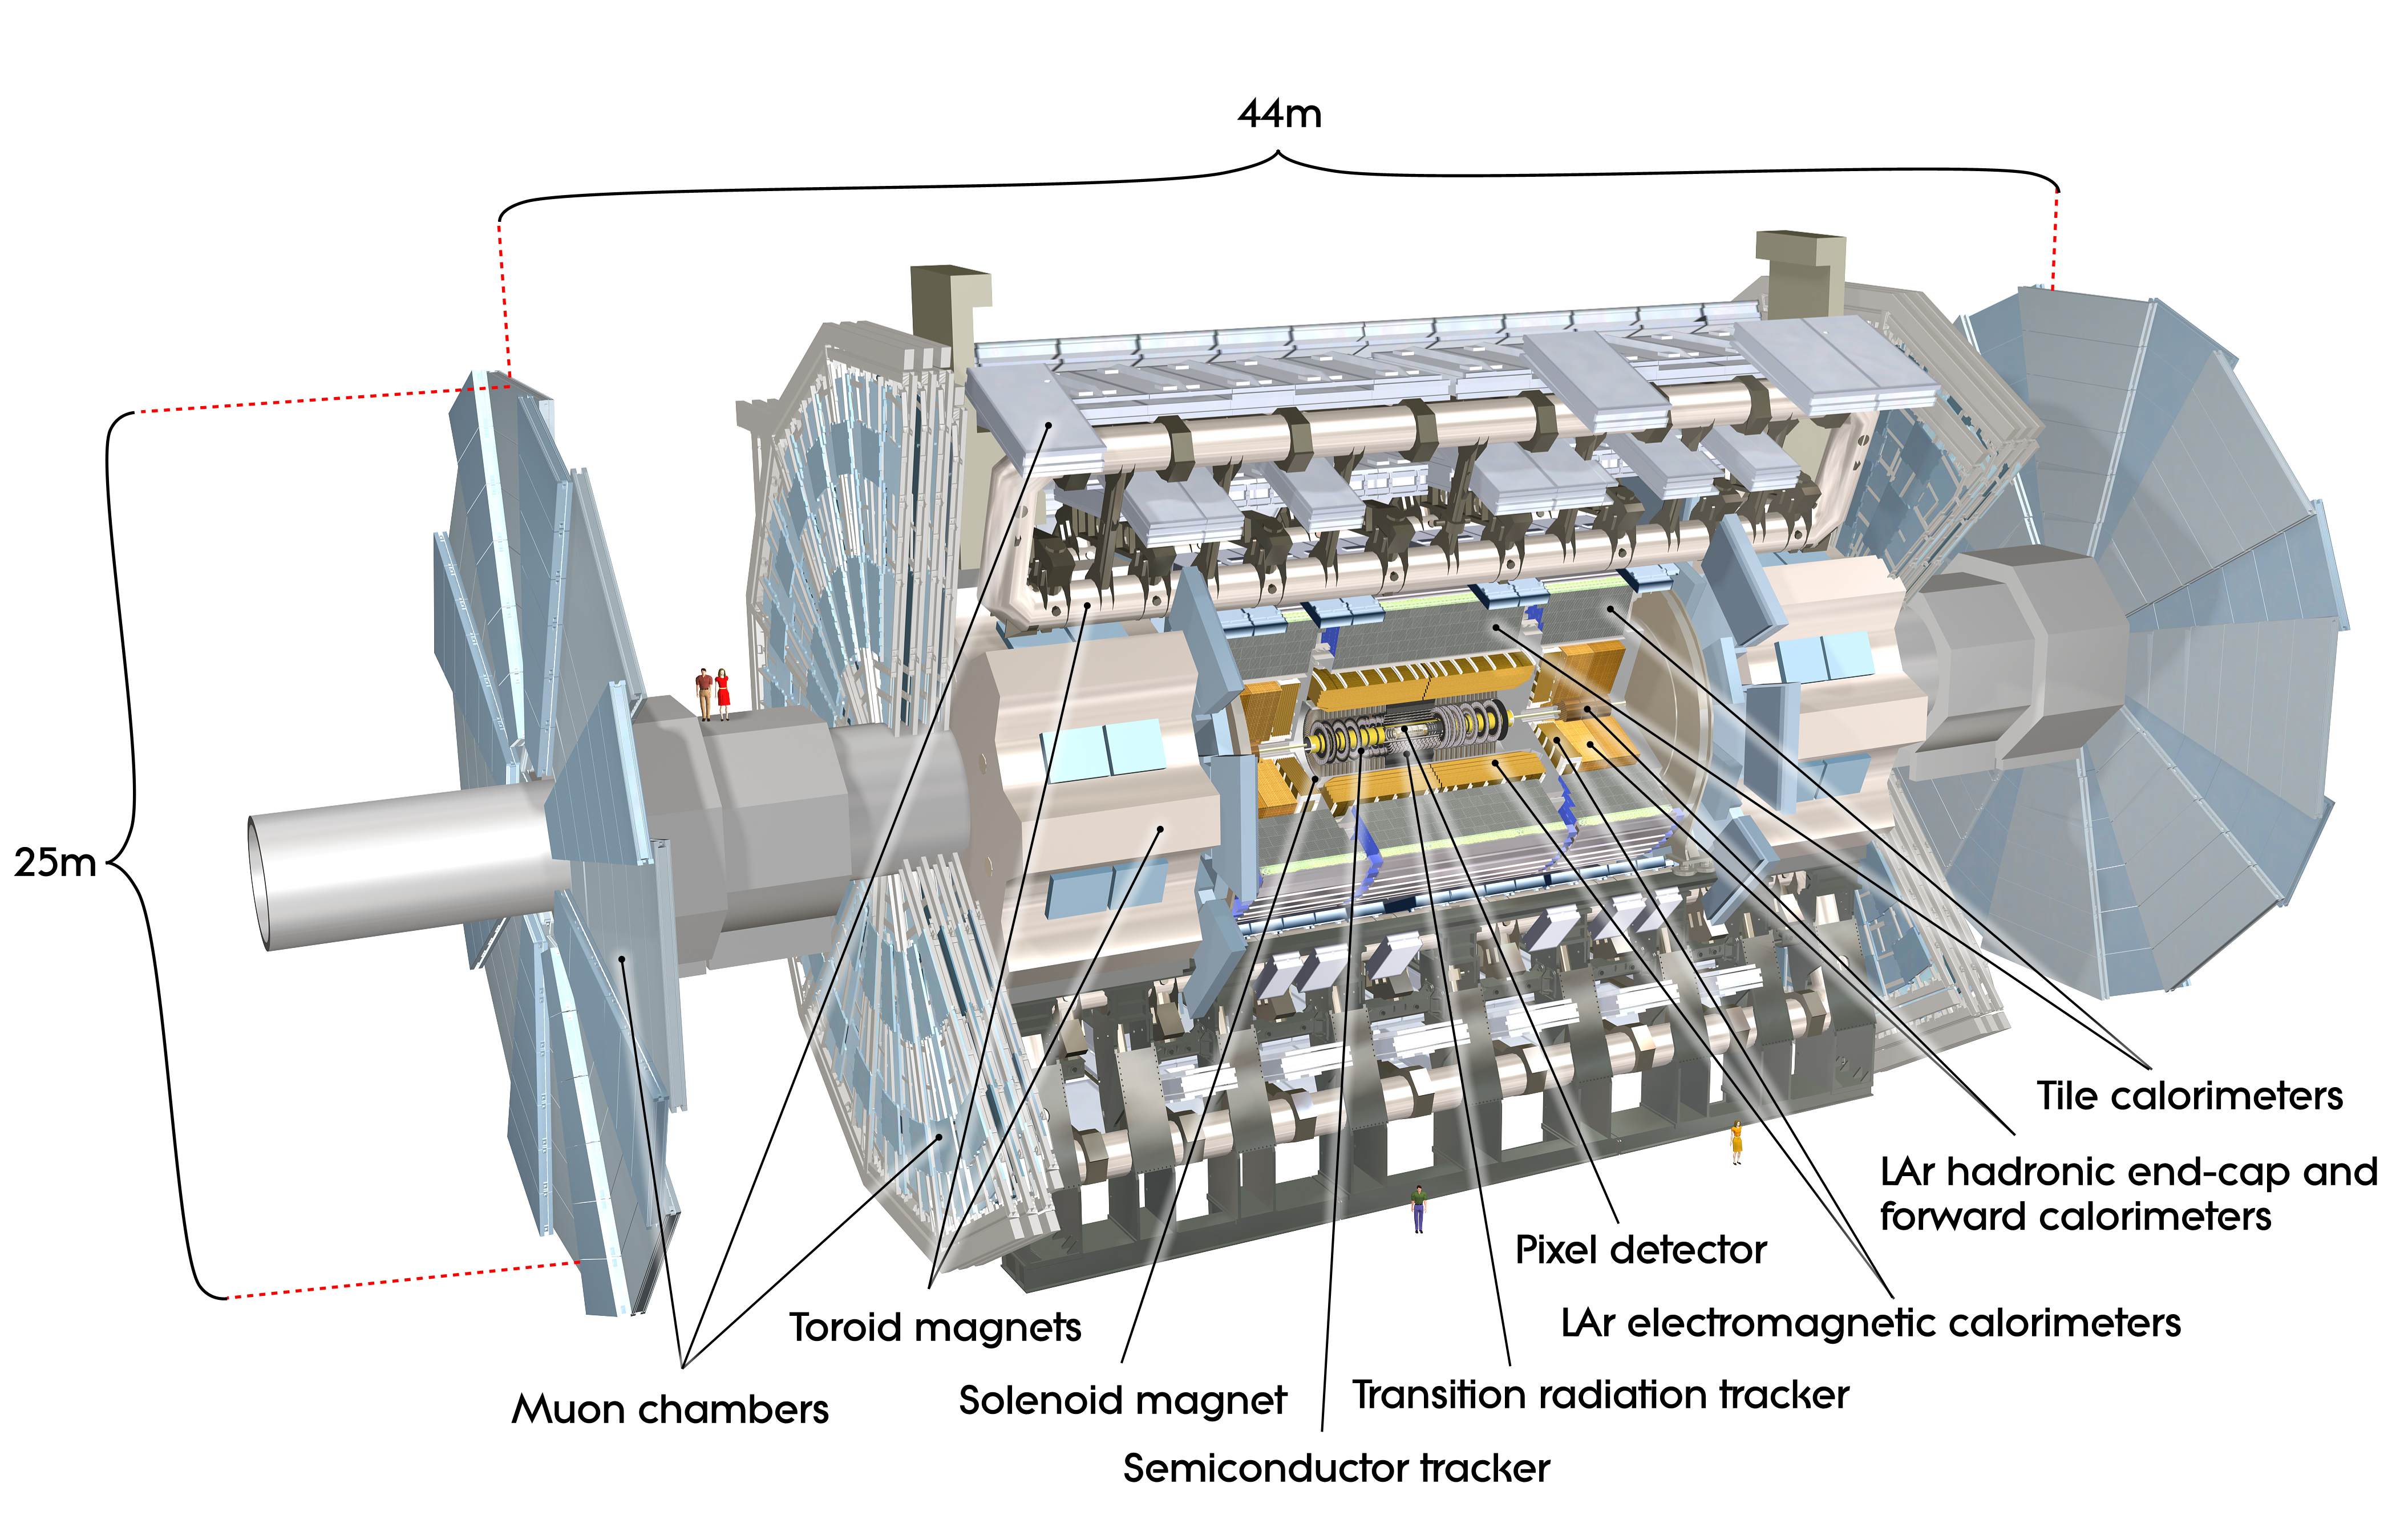
\includegraphics[width=.9\textwidth]{figures/atlas/detector.jpg}
\caption{A diagram of the ATLAS detector where the detector has
been artificially opened up to reveal the LHC beam line and the
various sub-detector components within. The sub-detector components
are labeled as such.}
\label{fig:atlas}
\end{figure}

%I need to define things here like eta, pt, deltaR, etc 
%I may need to talk about isolation here
The ATLAS detector~\cite{ATLAS} is designed to measure
the products of the particle collisions produced by the LHC.
In particular, the detector seeks to measure those stable 
(or meta-stable) particles whose decay lifetime is sufficiently
long enough to interact with the detector.  This includes
a variety of fundamental particles (like muons) as well as 
composite particles (like neutrons). The wide variety of 
particles to be measured requires the implementation
of several sub-detector systems that work in tandem 
to identify and measure their properties. 
A cylindrical geometry for the detector is chosen
which builds up around the beam line and surrounds
the collision point so that most of the collision
products will pass through it.
A diagram of the ATLAS detector can be seen in \fig\ref{fig:atlas}.
Its clydrincal shape is clear with a diameter of 25 meters
and length of 44 meters. The detector is massive, weighing
in at roughly 7000 tonnes; but it is also highly granular, with
over 100 million detection elements that are arranged very precisely, 
in many cases on the order of tens of microns.
In the ``opened'' view of \fig\ref{fig:atlas}, the proton-proton
collisions from the LHC occur at the core of the detector
and the sub-detector components build up around this point.

The detectable products of the collision pass outward from the collision
point through the different components where their energy and momentum
are measured. The way in which the particles interact with the various
sub-detector systems helps to identify the types of 
particles produced.
This can be more clearly seen in the diagram of 
\fig\ref{fig:atlas_wedge}, which shows how the most typical
products of the LHC collisions interact with the different
components of the ATLAS detector.
Nearest the collision point is the inner detector (ID), designed to 
measure the paths of charged particles passing through using several
different subsystems. This 
is surrounded by a 2 Tesla solenoidal magnet.
The field from the magnet bends the trajectory of charged particles
in order to measure their momentum.
Beyond that is the calorimeter system
which measures the energy deposits of all particles passing 
through (except for neutrinos). The calorimeter system 
itself is divided up into components which fall into two main 
categories: the electromagnetic (ECAL)
and hadronic calorimeter (HCAL) systems.
The ECAL is situated in front of the HCAL and is designed
primarily to absorb and mesasure the energy and position of
electrons and photons. 
The HCAL is designed to do the same for
composite particles like protons and neutrons.
Surrounding the calorimeter system is the muon spectrometer (MS),
which is the largest component of the ATLAS detector and the one
that determines its size. It is designed to quickly identify and measure the 
trajectory of muons as they pass through
and leave the detector using precision 
and triggering components. The MS is also composed of 
three large superconducting air-core toroid magnets 
which allow for
a measurement of the muon momentum. The neutrinos 
pass through without interacting.

\begin{figure}[ht!]
\centering
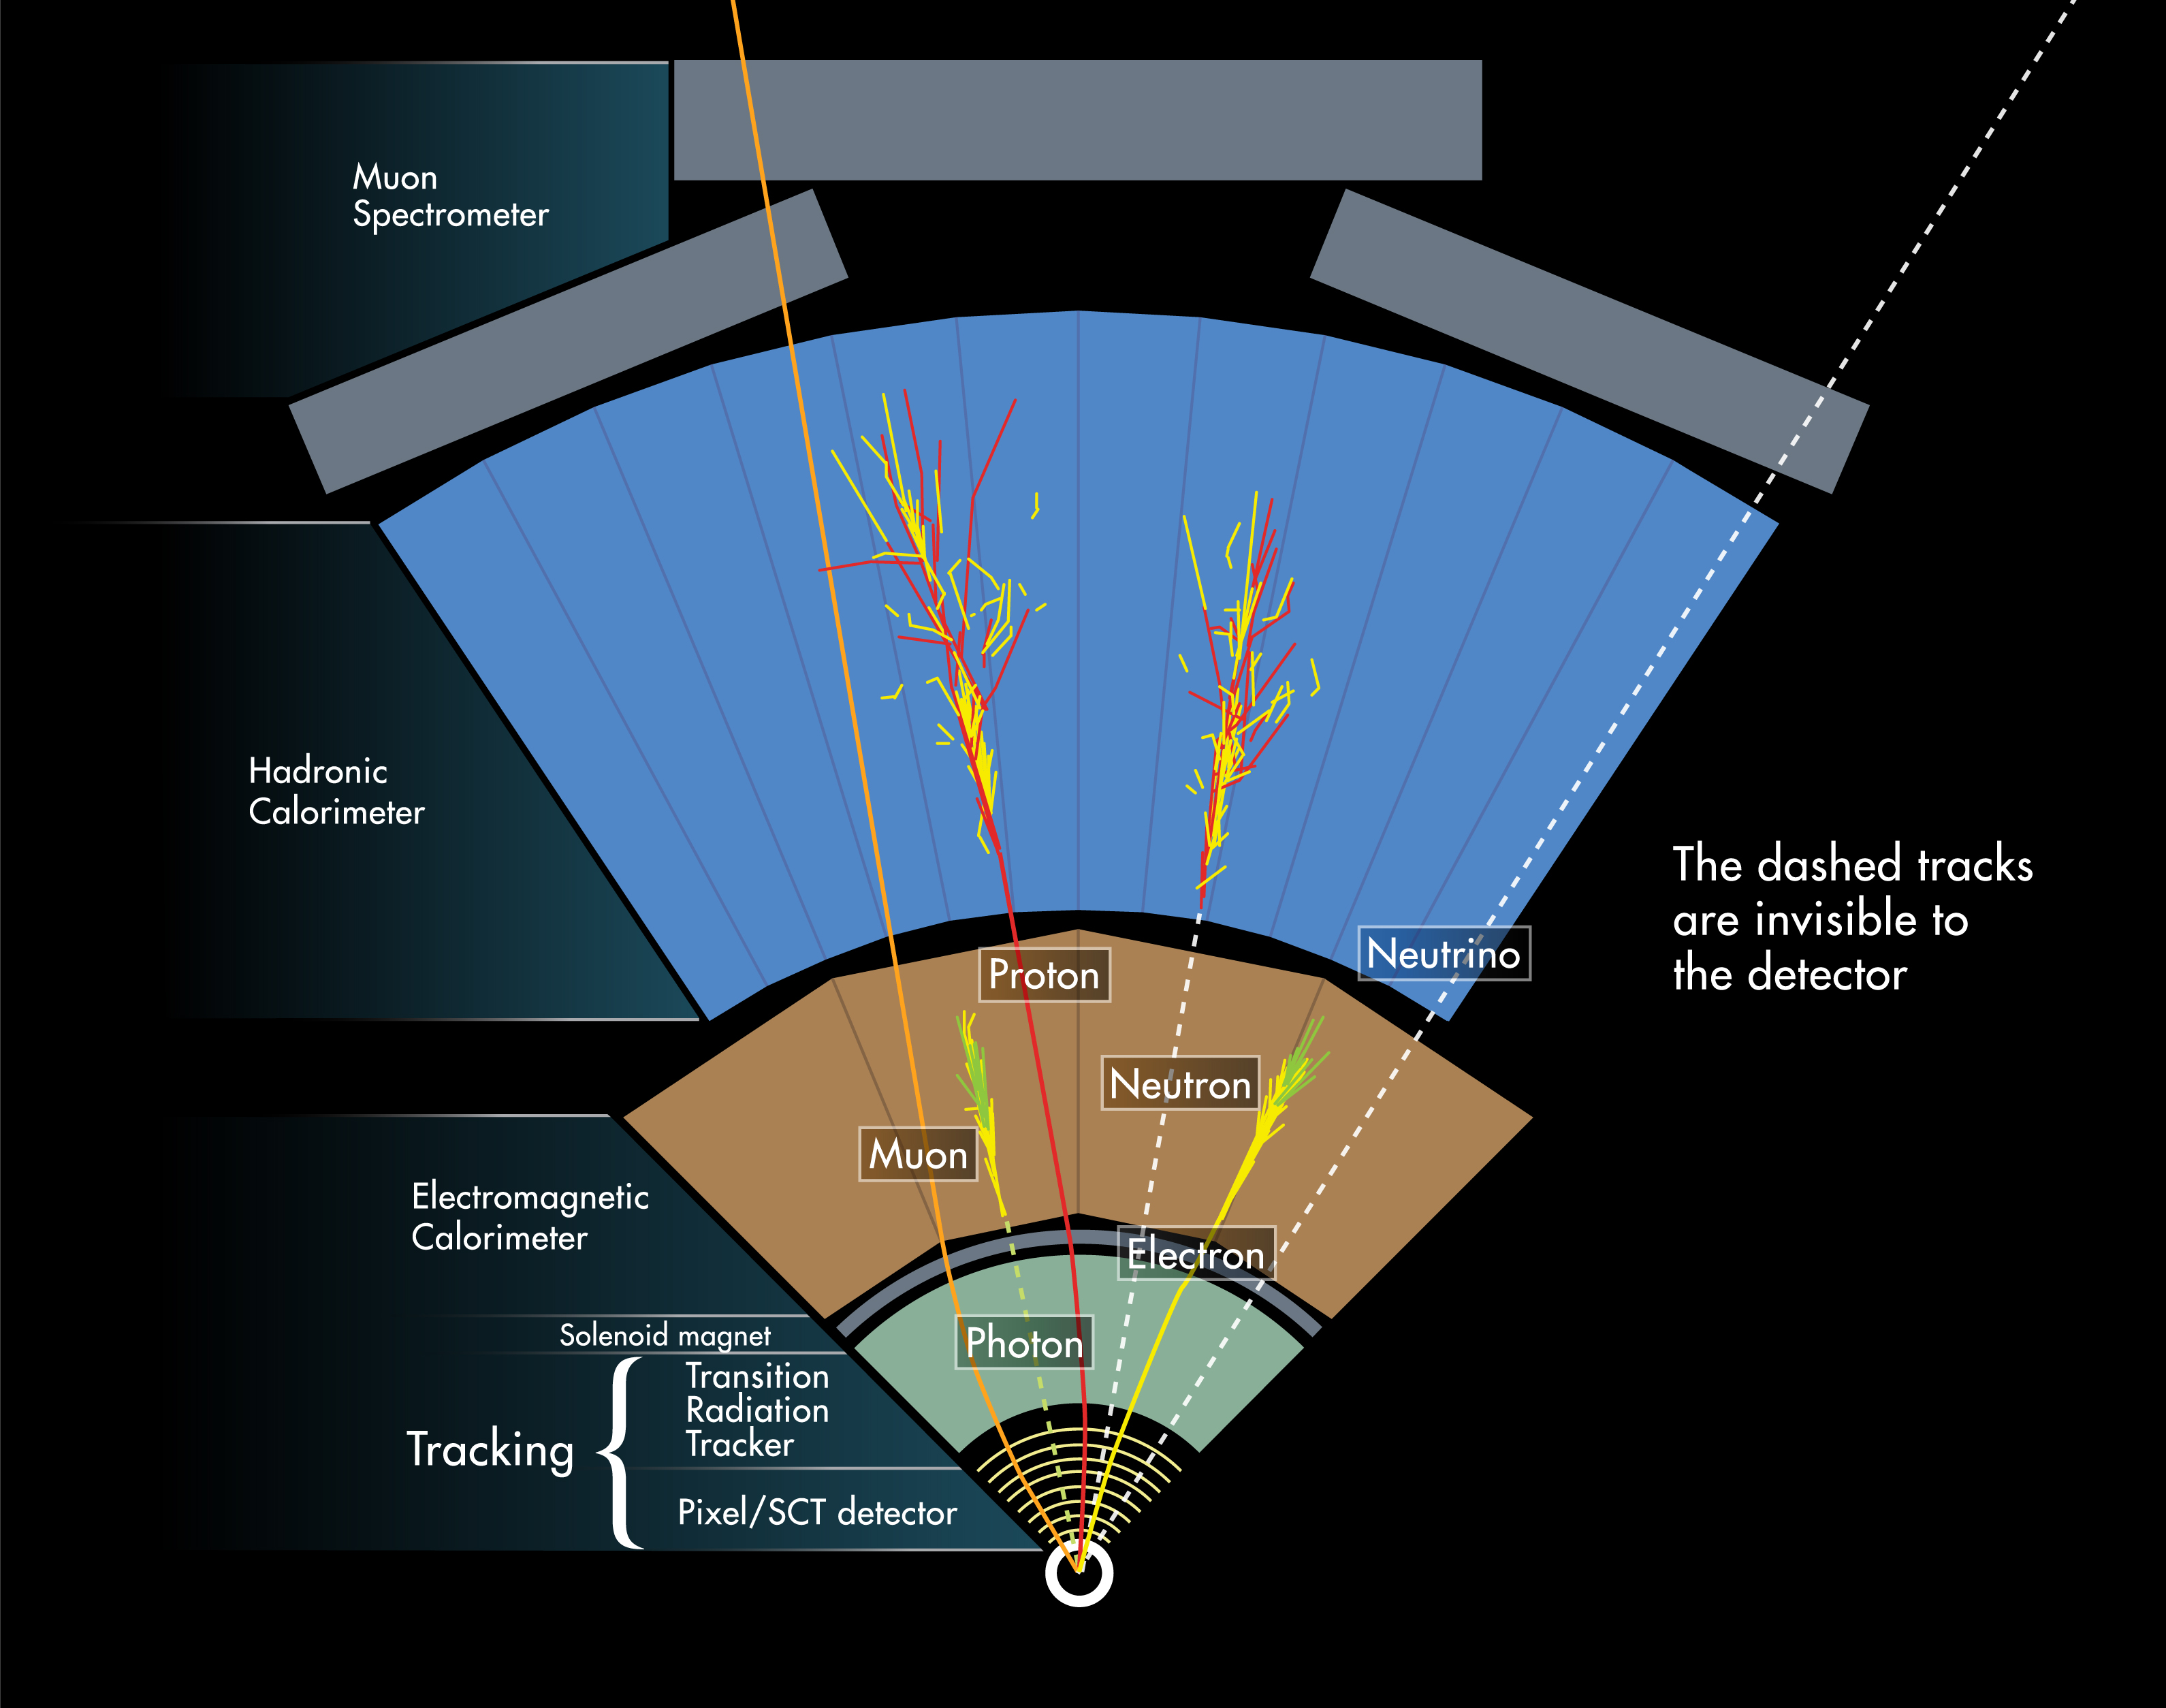
\includegraphics[width=.9\textwidth]{figures/atlas/wedge.jpg}
\caption{A diagram of one wedge of the ATLAS detector
as viewed from looking down the beam line. 
The sub-detector components are shown along with the 
particles that typically come from the collision.
The paths of the particles are shown to indicate how each particle 
interact with the detector.}
\label{fig:atlas_wedge}
\end{figure}

The geometry of the ATLAS detector is defined using a 
right-handed cylindrical coordinate system with the $x$-axis
pointing inwards towards the center of the LHC ring, the $y$-axis pointing
up, and the $z$-axis pointing along the beam-line, sometimes referred
to as the longitudinal or axial direction.
The $x-y$ plane, which is perpendicular to the beam-line,
is referred to as the transverse plane. In this plane, positions are  
defined using cylindrical coordinates with $r$ being the distance
from the beam-line and $\phi$ being the azimuthal angle.
The ATLAS detector has nearly uniform $2\pi$ 
coverage in $\phi$\footnote{The ID and calorimeter systems are designed
to have minimal cracks and roungly uniform coverage in $\phi$. The
spatial extent of the MS makes this challenging due to service
and support structures, thus there are cracks in the $\phi$ coverage in the MS.}.
For describing the direction of the particle with respect 
to the $z$-axis, a quantity called the rapidity, $y$,
can be related to the particle energy, $E$, and longitudinal momentum, $p_z$:
\begin{equation}
y = \frac{1}{2} \ln \Bigg(\frac{E+p_z}{E-p_z} \Bigg)
\end{equation}
whose distribution is invariant under Lorentz boosts in the longitudinal direction.
This is a useful characteristic as the longitudinal momentum of the
partons within the proton are not known on an 
event-by-event basis, as discussed in \sec\ref{sec:pdf}.
At the LHC, most stable particles 
are produced with energies much larger than their mass.
In this limit, 
the rapidity can be simplified to a quantity called the pseudo-rapidity, $\eta$:
\begin{equation}
\eta = -\ln \tan (\theta/2) 
\label{eq:pseudorapidity}
\end{equation}
which is only a function of the polar angle, $\theta$, 
the direction of the particle with respect to the positive $z$-axis.
The distribution of rapidity for the inclusive cross-section
at the LHC falls mostly within the ATLAS ID and MS detector volumes 
of $|\eta| < 2.5$ and $|\eta| < 2.7$, respectively, 
though the calorimeter system is extended out to $|\eta| < 4.9$
in order to ensure good coverage.

The transverse momentum of charged tracks can be determined by measuring how they 
bend in a magnetic field. The deviation of the trajectory
from a straight line path is referred to as the 
sagitta, $s$.\footnote{Technically, the sagitta, $s$, is defined in terms
of an arc as the distance from the center of the arc to the center of its
base. It can related to the radius of the arc, $r$, and the half the length
of the line connecting the two ends of the arc, $l$, by 
$s=r-\sqrt{r^2-l^2}$.} The sagitta is proportional to the magnetic
field strength and inversely proportional to the magnitude
of the particle's momentum in the transverse plane, known
as the transverse momentum or \pt.
Thus, a straight-line trajectory resembles an infinite-momentum charged
particle (or a neutral particle of any momentum), while
a bent trajectory corresponds to a charged particle with a finite momentum.
As a result, the transverse momentum resolution, $\Delta p_T$, is related to the 
precision on the measurement of the sagitta, $\Delta s$ by
\begin{equation}
\frac{\Delta p_T }{p_T} = \frac{\Delta s}{s}
\label{eq:sagitta}
\end{equation}
This also has the effect that the fractional uncertainty on the momentum
measurement grows linearly as a function of the momentum.


The total momentum of the proton-proton collision in the transverse
plane is nearly zero. Since the detector has nearly full azimuthal coverage 
in the transverse plane, we can test this constraint by measuring
the total trasverse momentum from the particles measured in the detector.
Thus, we may refer to this constraint as
\begin{equation}
\Bigg| \sum_{i\in\textrm{All Particles}} \vec{p}_{\textrm{T},i} \Bigg| = 0
\end{equation}
where the transverse momentum is added vectorialy and then
the magnitude is taken.
After adding up the $\pt$ of all of the particles to obtain
the total transverse momentum, 
any imbalance with respect to this constraint
is referred to as the
missing transverse energy, $\met$, and is attributed to the 
neutrinos produced in the collision. 
There is no such constraint on the longitudinal momentum of the partons
on an event-by-event basis
as discussed in \sec\ref{sec:pdf}.
This is the case
even though the momentum along the $z$-direction of the 
protons from which the partons are taken is, in fact, known.
Thus there is no direct way of determining with certainty the 
momentum of the neutrinos in the $z$-direction.



\section{Inner Detector}
\label{sec:atlas_id}

\begin{figure}[ht!]
\centering
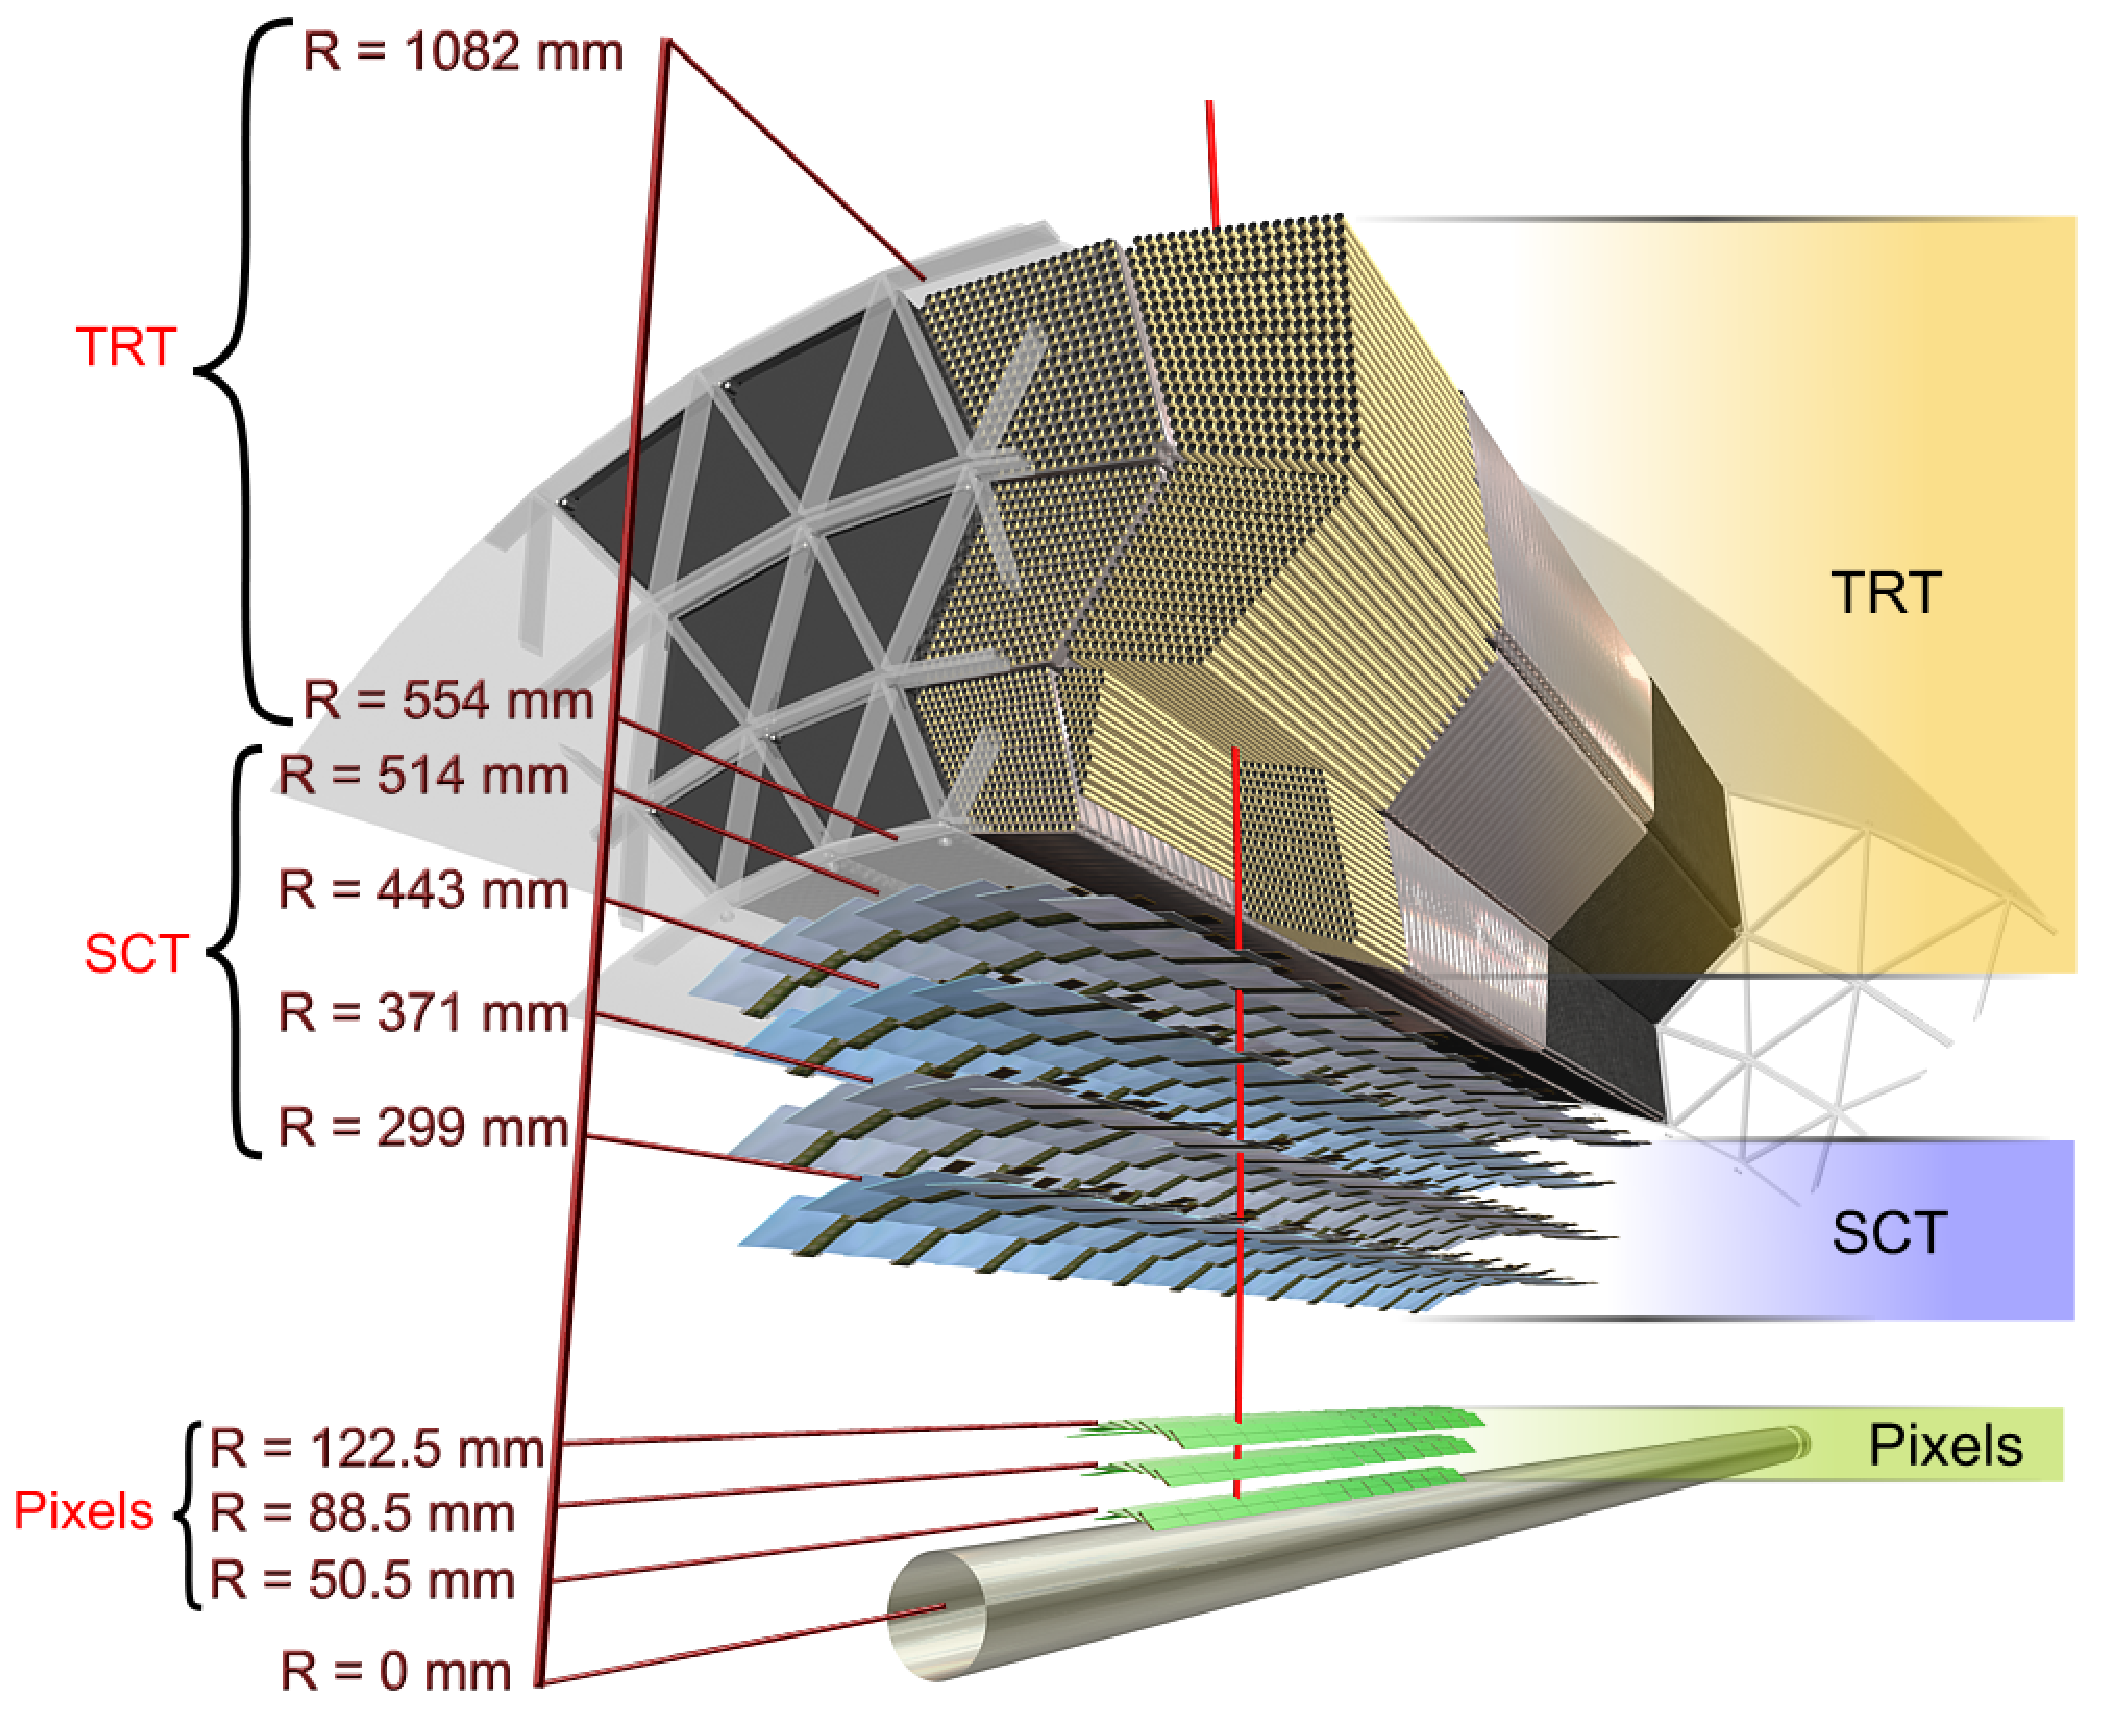
\includegraphics[width=0.7\textwidth]{figures/atlas/id_barrel.eps}
\caption{Diagram of the ATLAS Inner Detector (ID) system showing 
a wedge of the barrel system.  The three detector systems
are clearly labeled. The LHC beam pipe is axial to the system
and is shown at the bottom of the diagram.}
\label{fig:atlas_id_barrel}
\end{figure}

\begin{figure}[ht!]
\centering
\includegraphics[width=0.7\textwidth]{figures/atlas/id_endcap.eps}
\caption{Diagram of the ATLAS Inner Detector (ID) system showing 
a wedge of the endcap system as well as a part of the SCT and Pixel
barrel systems.  The detector systems
are clearly labeled.  The LHC beam pipe is axial to the system
but is not shown. Trajectories of two charged tracks 
with a $\pt=10\GeV$ are shown along $\eta=1.4$ and $\eta=2.2$ are shown 
by the solid bright red lines.}
\label{fig:atlas_id_endcap}
\end{figure}

The inner detector (ID) is the 
detector system that is closest to the beam pipe and thus the
first system that the products of the LHC collisions encounter
on their way from the collision point. Its primary role is 
to measure the trajectory and momentum of charged particles
through ionization as they pass through the detector.
It must be capable of measuring these tracks with high precision
in order to obtain precise momentum measurements and also to be able
to accurately extrapolate the tracks back to the collision point
to obtain primary and secondary interaction vertices with adequate
resolution for overcoming pileup 
conditions (see \sec\ref{sec:lhc_collider_physcs}). In addition,
since the system is so close to the LHC beam line, it
must be able to handle high particle fluxes. This requires that
the ID must have a very high granularity and fast electronics
readouts such that the occupancy of the
detector is small enough to distinguish individual tracks. In addition,
the detector materials and electronics must be sufficiently radiation
hard that they can withstand years of LHC 
exposure time\footnote{The layer of the pixel detector that is closest
the beam line is subjected to so much radiation that it is expected to be replaced
every three years.  Meanwhile, the radiation exposure of the other ID
components drops off rapidly (already by a factor of 6 for the third
pixel layer and by over a factor of 200 for the outer TRT) and is 
expected to survive for the planned lifetime of the detector.}.
The inner-most barrel layer of the pixel detector 
These tough requirements push the limits of available technology and thus
make the ID the most sophisticated detector system in ATLAS.



\begin{figure}[ht!]
\centering
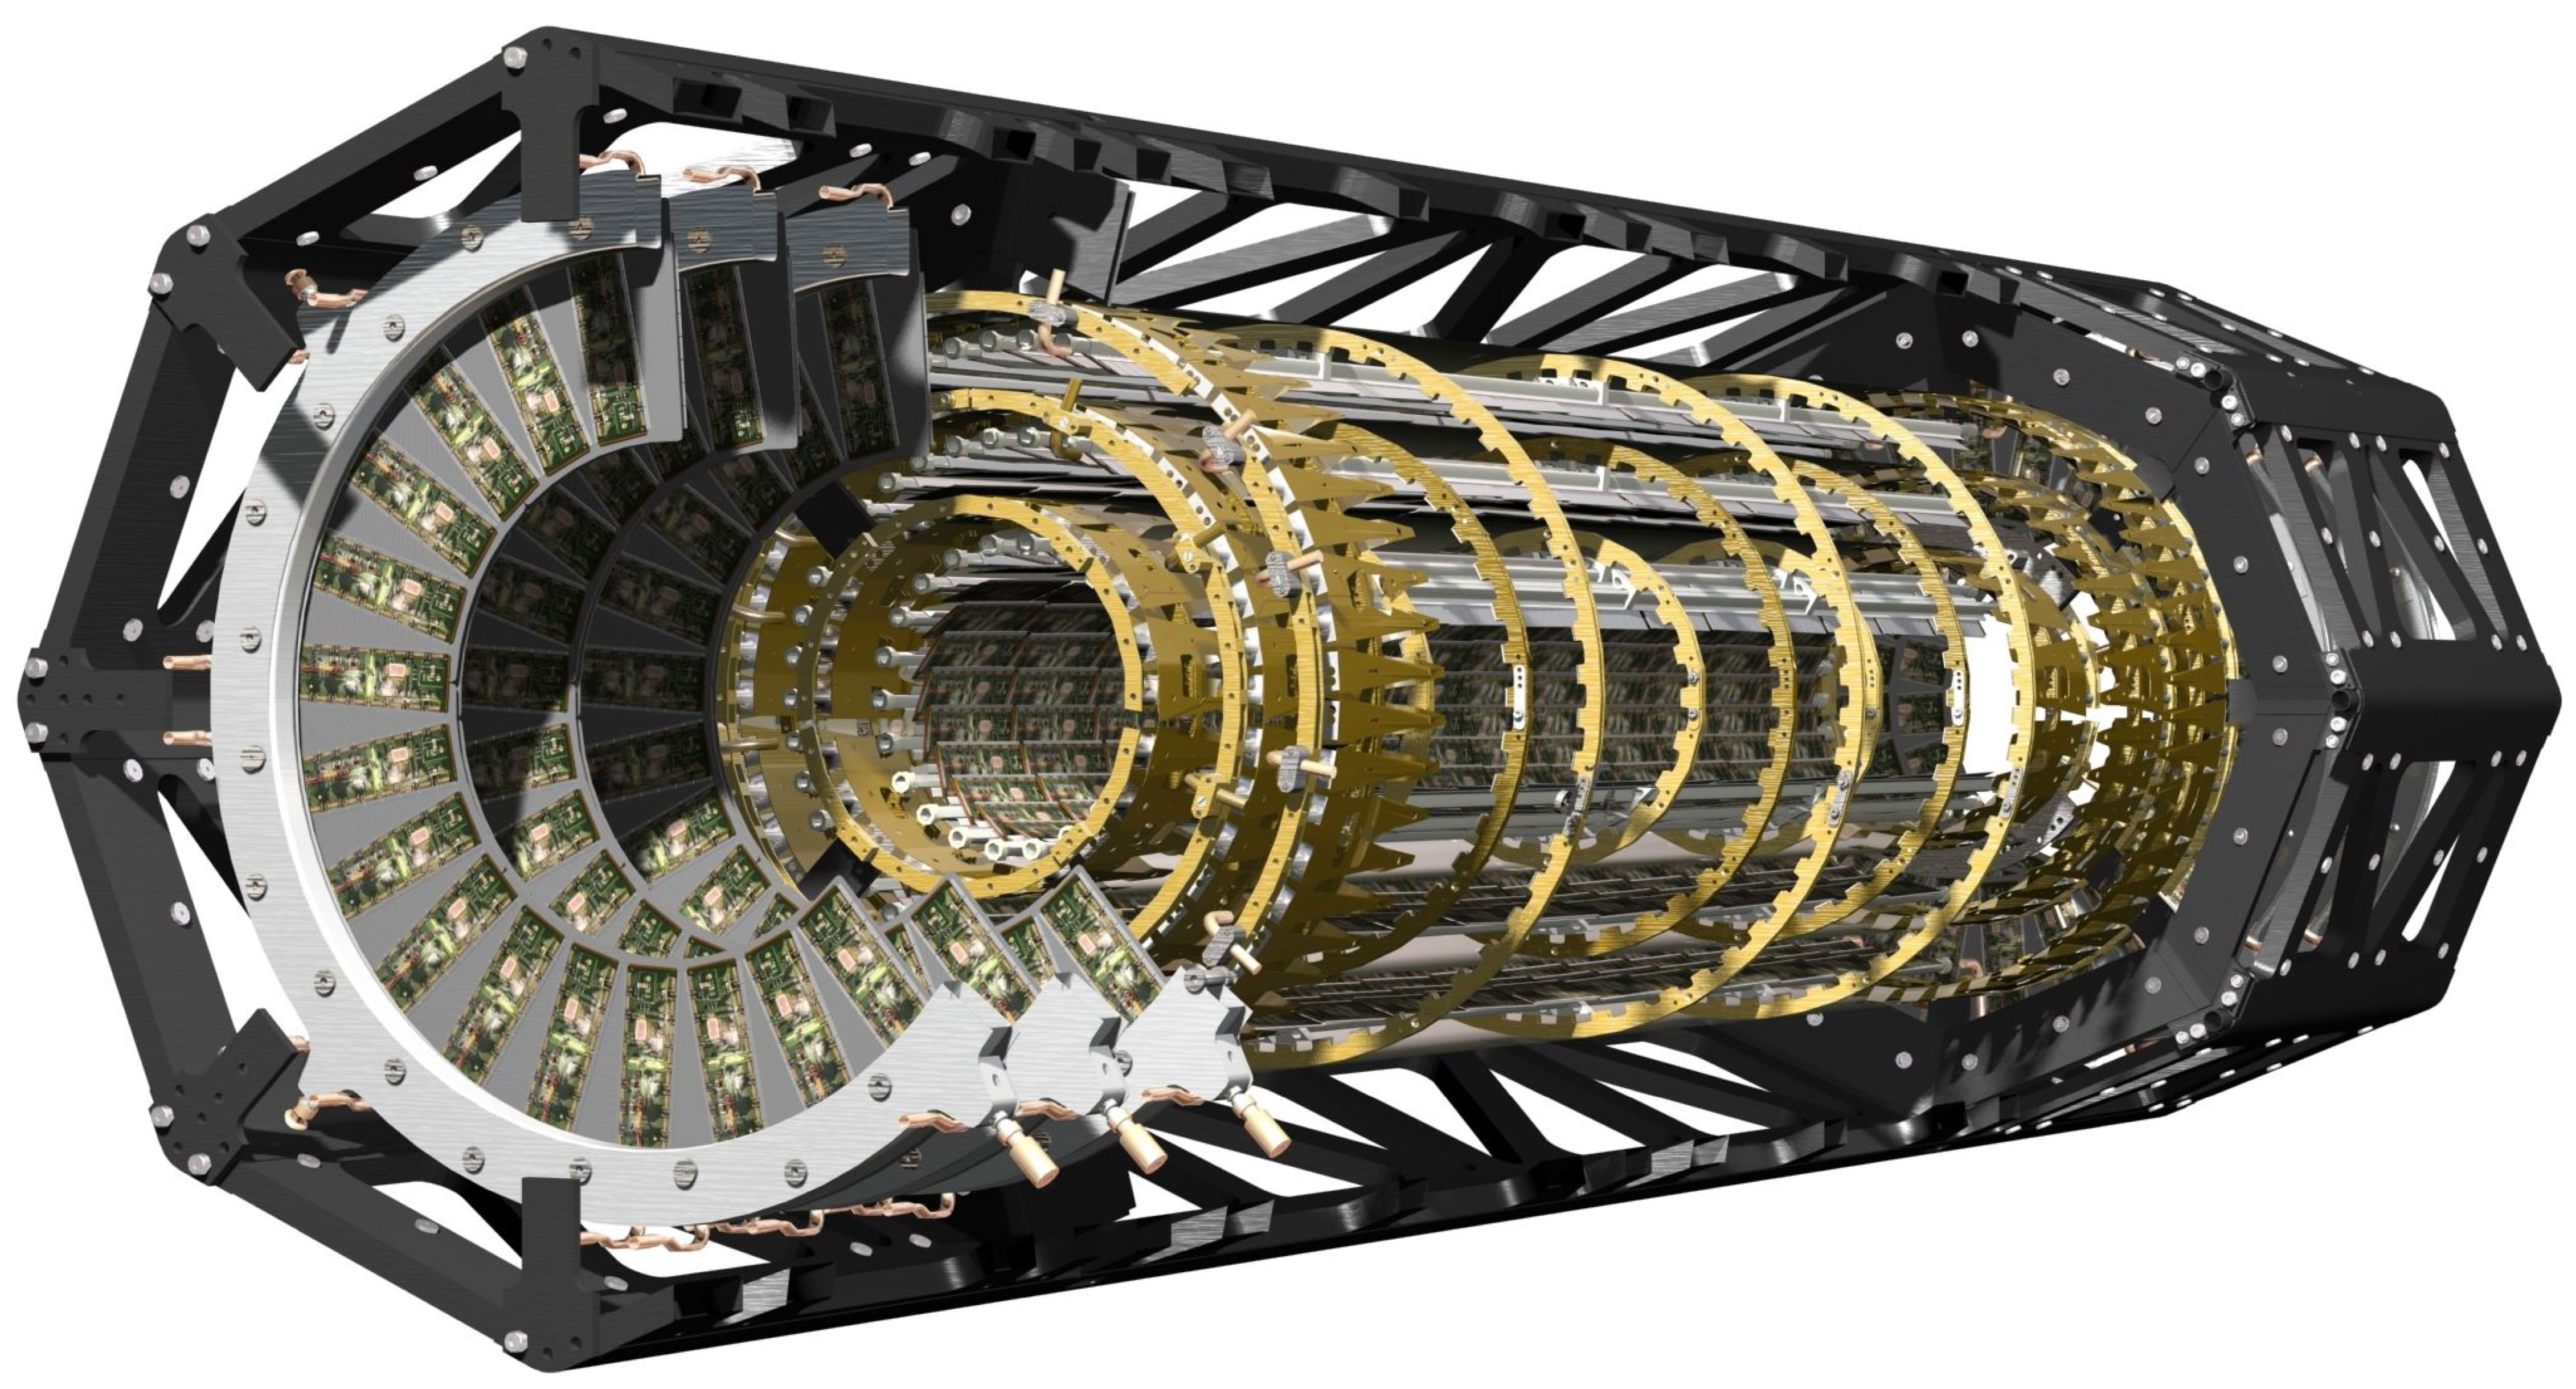
\includegraphics[width=0.7\textwidth]{figures/atlas/pixel.eps}
\caption{A cut-out diagram of the ATLAS pixel detector showing 
the arrangement of the pixel modules (green) in three layers of the barrel
and three layers of one end-cap system. Some of the support structure is
also shown.}
\label{fig:atlas_pixel}
\end{figure}

There are three different detector subsystems within the ID, together
immersed in a uniform 2 Tesla axial magnetic field: the pixel detector,
the silicon microstrip (SCT) detector, and the transition radiation
tracker (TRT). These three detector systems can be seen 
in the barrel in \fig\ref{fig:atlas_id_barrel} and from an alternate
view also showing one of the end-caps in \fig\ref{fig:atlas_id_endcap}. 
The pixel detector
is composed of more than seventeen hundred thin doped silicon sensors with 
dimension $19\times 64~\textrm{mm}^2$. Each sensor has more than forty-six
thousand readout elements (with a 
nominal size of $50 \times 400 \mu\textrm{m}^2$),
corresponding to the ``pixels'' which give the detector its name. 
A charged particle passing through an individual pixel produces a signal
which identifies the location of a charged particle. The combination of 
several layers can thus be used to form the trajectory of the particle. %sagitta
Each sensor is attached to a single readout electronic board, which comprises
one module.
The modules are arranged into three cylindrical barrel layers (at 
$r = $ 51 mm, 89 mm, and 120 mm)  and 
two end-caps each with three disk-shaped layers (at $z = $ 500 mm, 580 mm, 
and 650 mm) such that there is uniform
azimuthal coverage. A cut-out diagram of the pixel detector 
structure with modules in place in both the barrel and end-caps is shown 
in \fig\ref{fig:atlas_pixel}. The barrel covers roughly 
$|\eta|<1.7$ and the two end-caps roughly $1.7<|\eta|<2.5$.
Test beam measurements show that the 
spatial resolution of the pixel detector is around $12~\mu\textrm{m}$ in 
the $R-\phi$ plane and is slightly degraded orthogonal to this plane.



The SCT uses almost sixteen thousand thin silicon strip sensors, though not of the 
same type as in the pixel detector. 
A barrel silicon strip sensor has dimension $6.36\times 6.40~\textrm{cm}^2$
with 768 readout strips running along the longer dimension. The barrel
strips are placed in four concentric cylindrical layers, uniformly in azimuth
(at $r = $300 mm, 370 mm, 440 mm, and 510 mm),
the strips aligned axially with a strip pitch of 
80 $\mu$m, and covering roughly
$|\eta|<1.4$, as can be seen in \fig\ref{fig:atlas_id_barrel}.
In each of the two end-caps the sensors are made to form nine
disks spaced apart along the axial 
direction (at $z = $0.85 m, 0.93 m, 1.1 m, 1.3 m, 1.4 m, 
1.8 m, 2.1 m, 2.5 m, and 2.7 m) covering roughly $1.4 < |\eta|<2.5$, 
as seen in \fig\ref{fig:atlas_id_endcap}. The strips are similar
to the barrel except that they are tapered along the strip direction.
The sensors are then oriented such that the taper expands radially outward
with a strip pitch ranging from 60 $\mu$m to 90 $\mu$m as $z$ increases, 
In a test beam, the spatial resolution is found to be about $16~\mu\textrm{m}$
in the $R-\phi$ plane. Due to the length of the strips, the precision is considerably
worse in the axial direction for the barrel and the radial direction for 
the end-caps, with a precision of roughly $580~\mu\textrm{m}$.


The TRT uses a fundamentally different technology 
than the pixel and SCT.
Drift tubes are used of 4~mm in diameter 
which are filled with a Xenon-based gas mixture
and with an anode wire running through the center.
The tubes can be placed in close
proximity such that many measurements, around 36,
can be made on a single charged track. Another important feature
of the TRT is its ability to identify electrons using transition radiation.
This is achieved by surrounding the tubes in polypropylene material to induce
transition radiation from incident particles and taking advantage
of the discrimination power of the Xenon-based gas between 
transition radiation and tracking signals.
For electrons with $\pt>2\GeV$, usually 7 to 10 hits due to transition
radiation will be measured.
The barrel TRT runs from roughly $|\eta|<0.7$ and
is constructed from 144 cm long straws aligned
axially. Over fifty-two thousand straws are interleaved
with polypropylene fibers to form 73 layers of straws 
spaced roughly 7 mm apart and surrounding the beam-pipe with
a cylindrical symmetry and uniform coverage in azimuth,
as seen in \fig\ref{fig:atlas_id_barrel}.
In each of the two end-caps, two wheels are formed from over seventy-three
thousand straw tubes, 37 cm in length, 
oriented and distributed uniformly in azimuth. 
The inner wheel is formed from twelve layers and the outer wheel from eight
layers of straws spaced 8 mm and 15 mm apart, respectively,  
with 768 straws per layer, seen in \fig\ref{fig:atlas_id_endcap}.
The end-caps cover roughly $0.7<|\eta|<2.2$.
An individual straw has a precision of about $170~\mu\textrm{m}$ along
its diameter.




efficiency of electron identification?


large number of readouts?
occupancy??
noise??
sagitta???
explain how the b-field is used?
eta coverage?
materials?
electronics?
more figures?



\section{Calorimeters }
\begin{figure}[ht!]
\centering
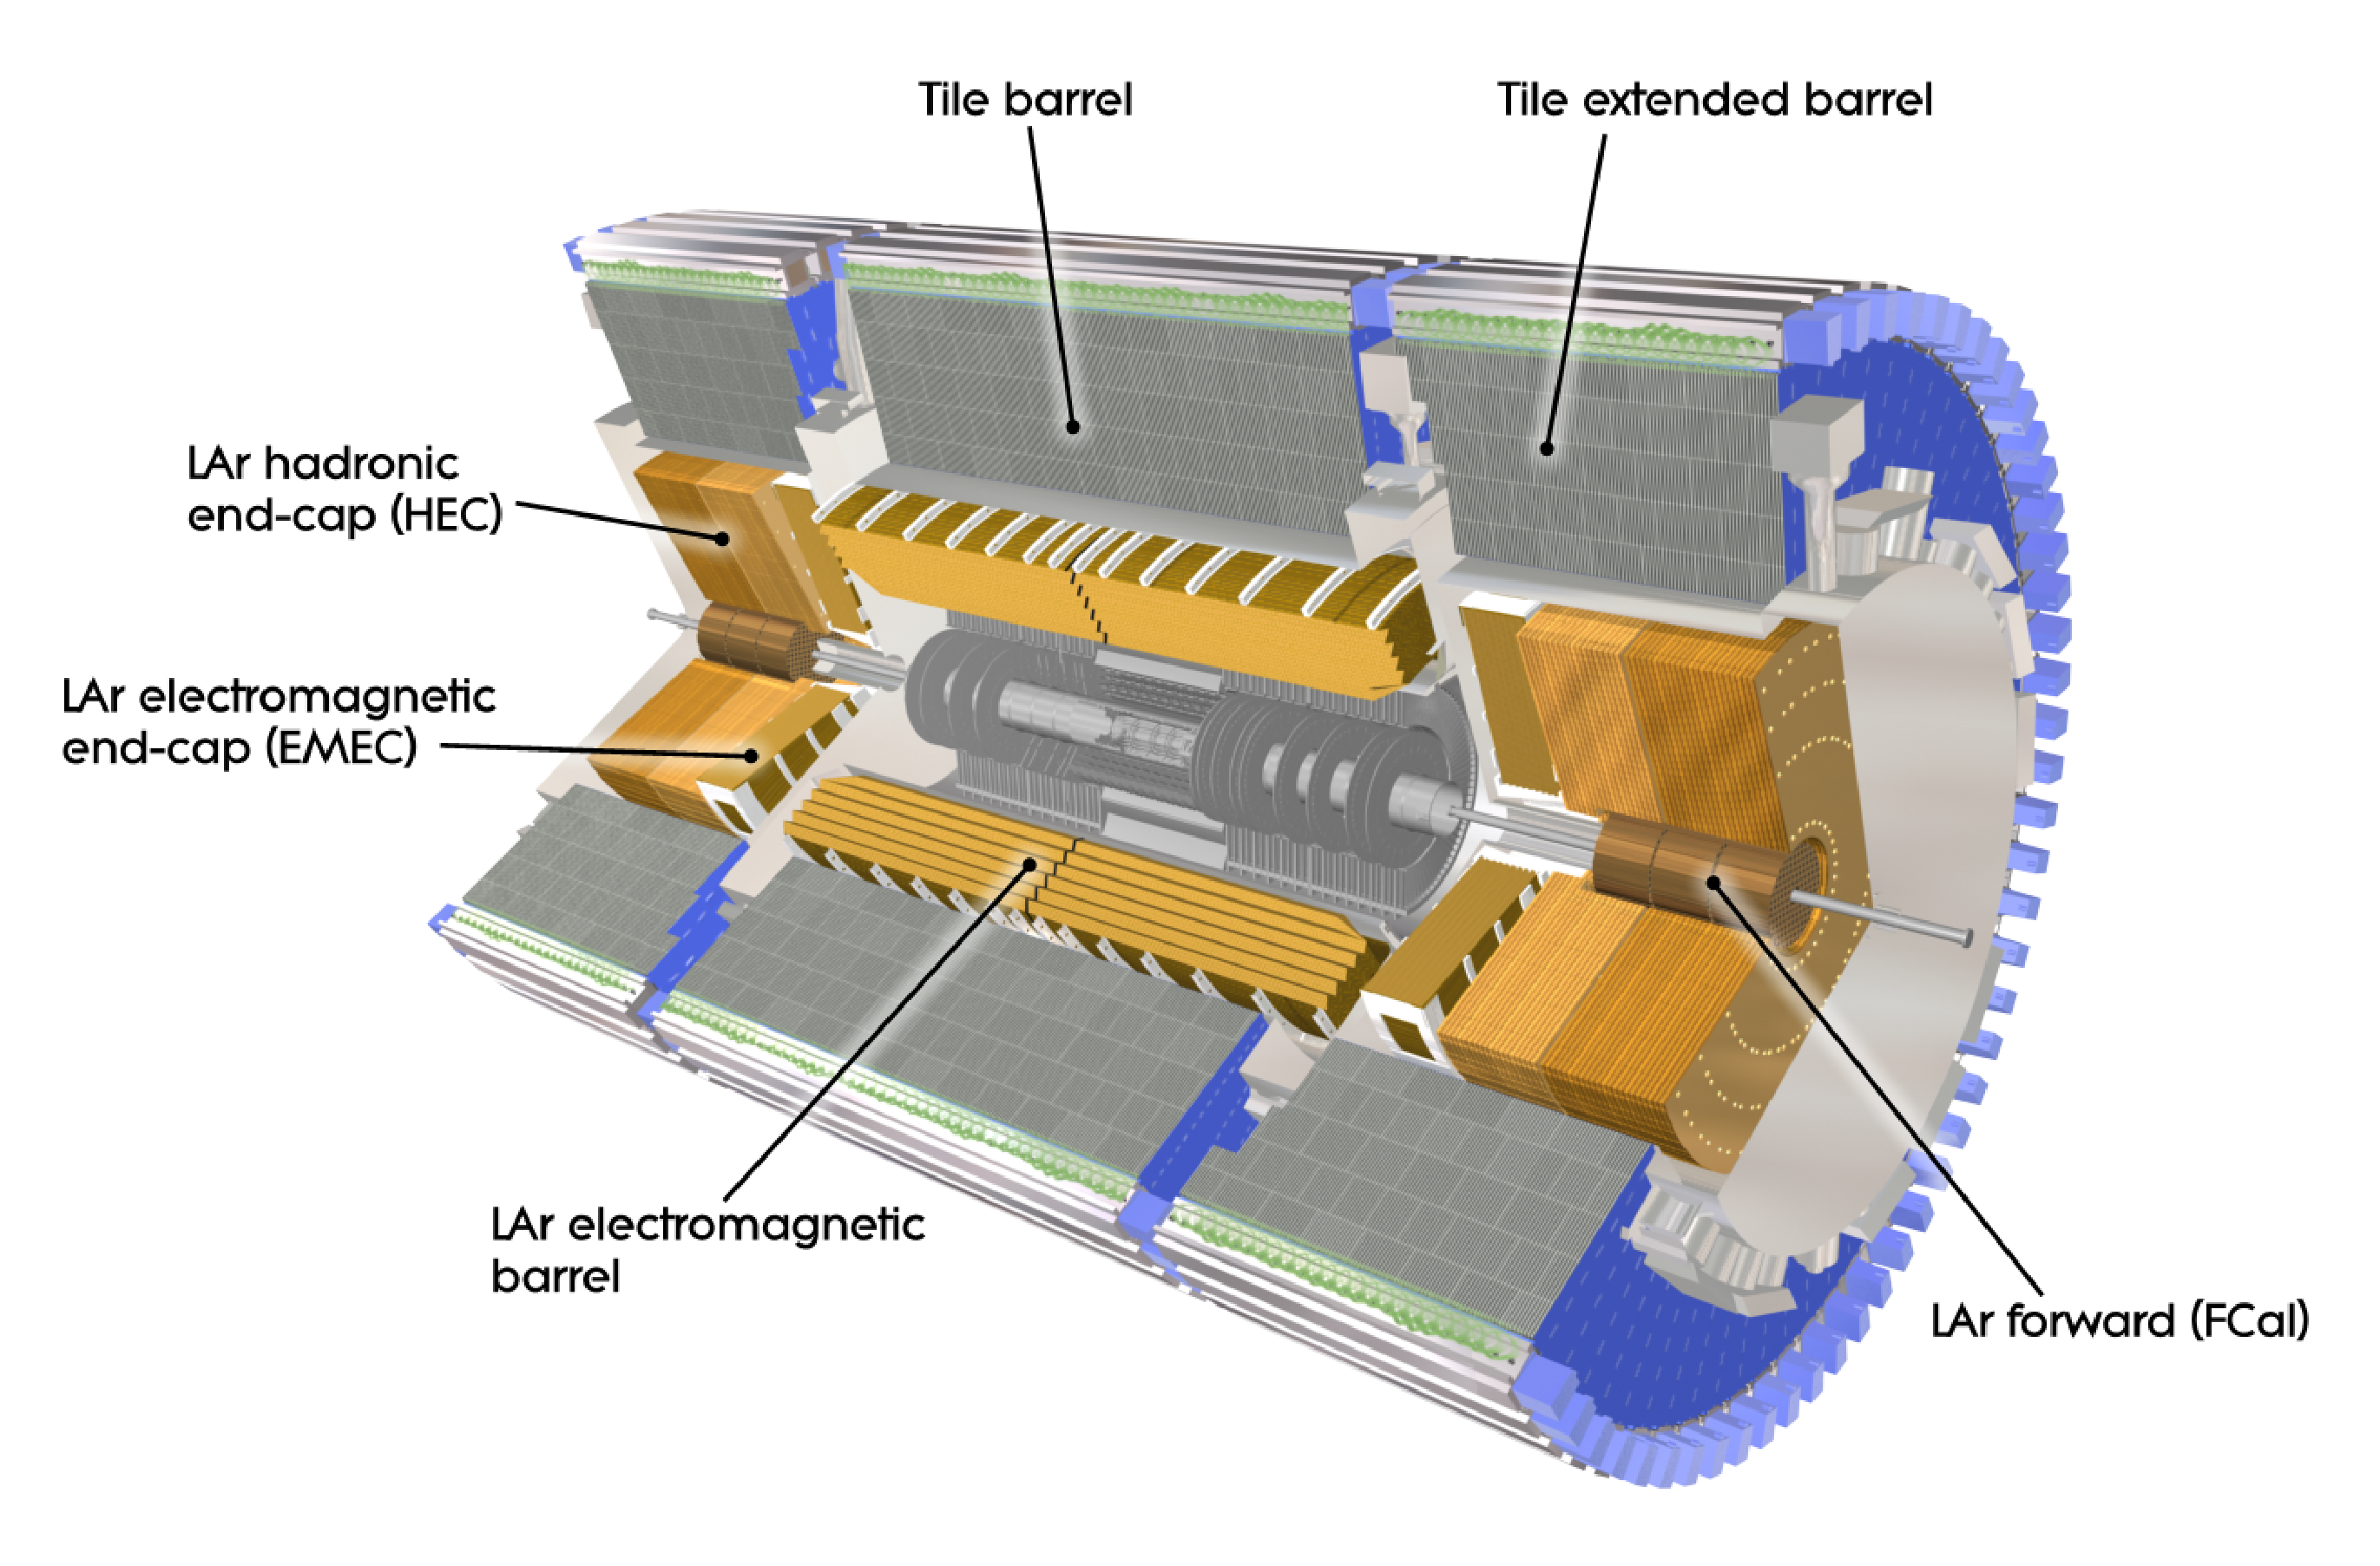
\includegraphics[width=0.9\textwidth]{figures/atlas/calorimeter.eps}
\caption{Diagram of ATLAS calorimeter system with cut-out portion
to allow a view of the nested sub-components.}
\label{fig:atlas_calorimeter}
\end{figure}


\begin{figure}[ht]
\centering
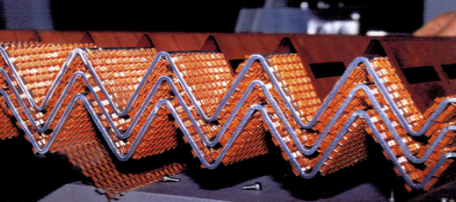
\includegraphics[width=.5\textwidth]{figures/atlas/emcal_accordion.png}
\caption{Photo of three ECAL sampling layers
showing the ``accordion'' structure. In the picture, 
the horizontal directions corresponds to 
the radial direction when the detector is in position, which is
the direction the LHC products would follow.}
\label{fig:atlas_emcal_accordion}
\end{figure}

\begin{figure}[ht]
\centering
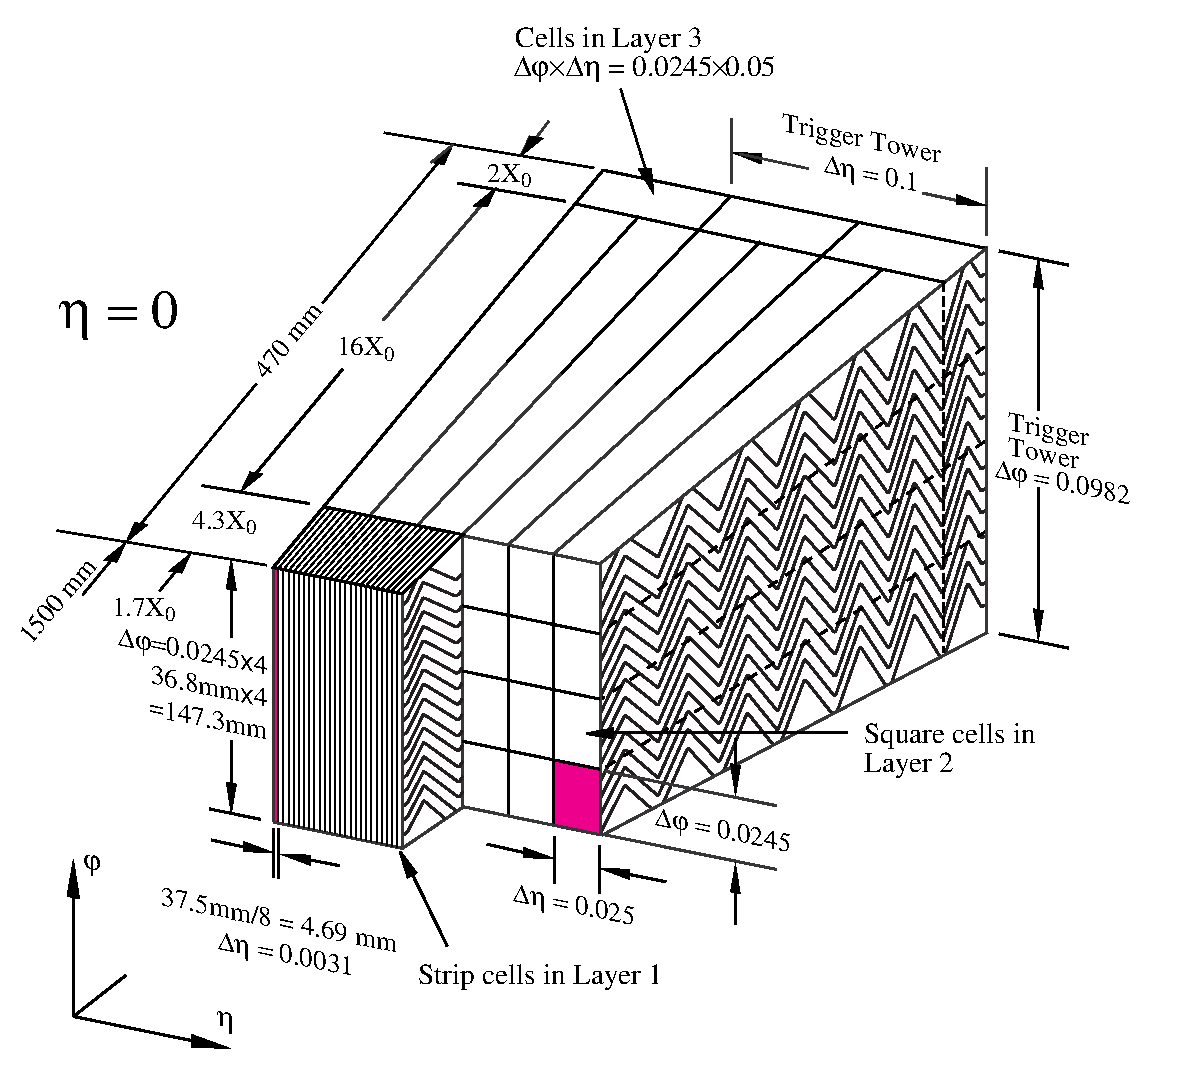
\includegraphics[width=.8\textwidth]{figures/atlas/emcal_barrel_module.eps}
\caption{ A diagram of one ECAL barrel module 
covering $22.5^{\circ}$ in azimuth.}
\label{fig:atlas_emcal_module}
\end{figure}

The ATLAS calorimeter is designed to measure the energy
deposits of the products of the LHC collisions which pass through
it except for the neutrinos.  A diagram of the 
calorimeter system can be seen in \fig\ref{fig:atlas_calorimeter}.
The calorimeter system is split into four main systems, 
the electromagnetic calorimeter (ECAL), the 
tile hadronic calorimeter (HCAL), the hadronic 
end-cap calorimeter (HEC), 
and the Forward Calorimeter (FCAL).
The ECAL is a sampling calorimeter that uses lead as the sampling
medium and liquid Argon (LAr) as
the active medium from which the charge of the electromagnetic
shower produced by incident particles on the sampling medium
can be collected.  LAr is used as the active medium 
because of its radiation hardness and its linear response.
%as evidenced in \fig\ref{fig:atlas_emcal_response}.
The lead sampling medium alternates with the active LAr medium
using lead plates 1-2~mm thick with an approximately 4~mm 
LAr gap between each sheet and electrodes placed in the middle of
the gaps.
The lead sheets are constructed using a unique ``accordion'' structure,
as seen in \fig\ref{fig:atlas_emcal_accordion}. 
This is to provide a uniform resolution with no gaps
in the azimuthal direction.
The ECAL itself can be split up into a barrel region ranging
from $0<|\eta|<1.3$ and two end-cap regions ranging from 
$1.5 < |\eta| < 3.2$.
The thickness of the barrel region in units of radiation length, \xzero,
ranges from $22~\xzero$ to $30~\xzero$
for $|\eta|<0.8$ and from $24~\xzero$ to $33~\xzero$ for
$0.8 < |\eta| < 1.3$.
The barrel region is divided into individual modules
which together surround the beam-line
in a cylindrical shape.  A diagram of one such module
can be seen in \fig\ref{fig:atlas_emcal_module}.
From this one can see that each module is segmented in $\eta$
and $\phi$, as well as into three layers in depth.
The segmentation is applied to obtain pointing information, 
which aids in the identification and measurement of electromagnetic
objects in conjunction with measurements from the ID.
The very fine segmentation in $\eta$ of the first layer
in depth is important for precision tracking measurements.
The second layer has a larger depth and thus collects most of the energy.
There are two identical end-cap regions, one on each side of the 
collision point. Each end-cap region consists of two wheels: the 
outer wheel from $1.4756 < |\eta| < 2.5$, with a thickness ranging from
$24~\xzero$ to $38~\xzero$, and 
the inner wheel from $2.5 < |\eta| < 3.2$, with a thickness ranging from
$26~\xzero$ to $36~\xzero$.
The regions from $1.5 < |\eta|<2.5$ in the inner and outer wheels both
have three layers, with the first being a finely segmented precision
layer similar to the barrel regions. Outside this region there 
are only two layers with a coarser segmentation.
The ECAL also consists of a pre-sampler detector with a single layer of LAr in 
front of the full barrel ECAL and in front of the end-cap ECAL calorimeters
from $1.5 < |\eta| < 1.8$; this aids in the measurement of the energy deposits
prior to reaching the ECAL and allows 
for a better understanding of the energy deposited
in the transition region between the barrel and end-caps.


\begin{figure}[ht]
\centering
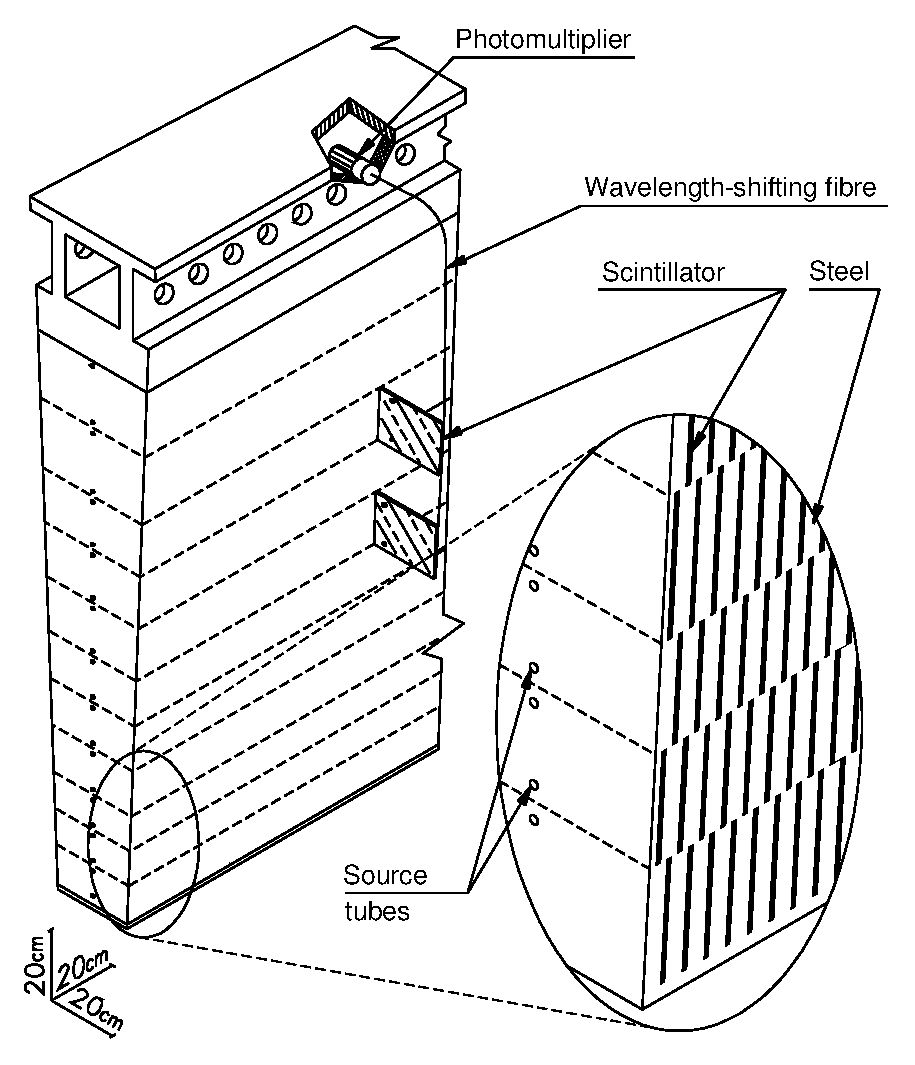
\includegraphics[width=.6\textwidth]{figures/atlas/hcal_module.eps}
\caption{ A diagram of one tile HCAL module 
covering $5.625^{\circ}$ in azimuth. The radial direction when 
positioned in the detector corresponds to the vertical direction in the
image.}
\label{fig:atlas_hcal_module}
\end{figure}


The tile HCAL is a steel sampling calorimeter with scintillating tiles used as the 
active material.
Steel is chosen as the sampling material since it gives a good
depth in interaction lengths, $\lambda$, with a maximum depth
of $7.4~\lambda$, while also having a low cost.
It is split into a central barrel and two extended barrels 
which together cover a 
region from $|\eta|< 1.7$, as can be seen in \fig\ref{fig:atlas_calorimeter}.
As in the ECAL barrel, the tile HCAL is divided into individual modules
that surround the collision point in azimuth; a diagram of one such
module is shown in \fig\ref{fig:atlas_hcal_module}.
The scintillating tiles alternate periodically with the self-supporting
steel body and are oriented radially. 
The scintillation
light is routed through wavelength-shifting fibers and collected
at photo-multiplier tubes placed at the back of the module.
This configuration allows for a near uniform coverage in azimuth.  
In the crack region from $1.2 < |\eta| < 1.6$ between the central barrel 
and extended barrels, special modules are placed to recover and correct
for energy losses in this region.

\begin{figure}[ht] 
\centering
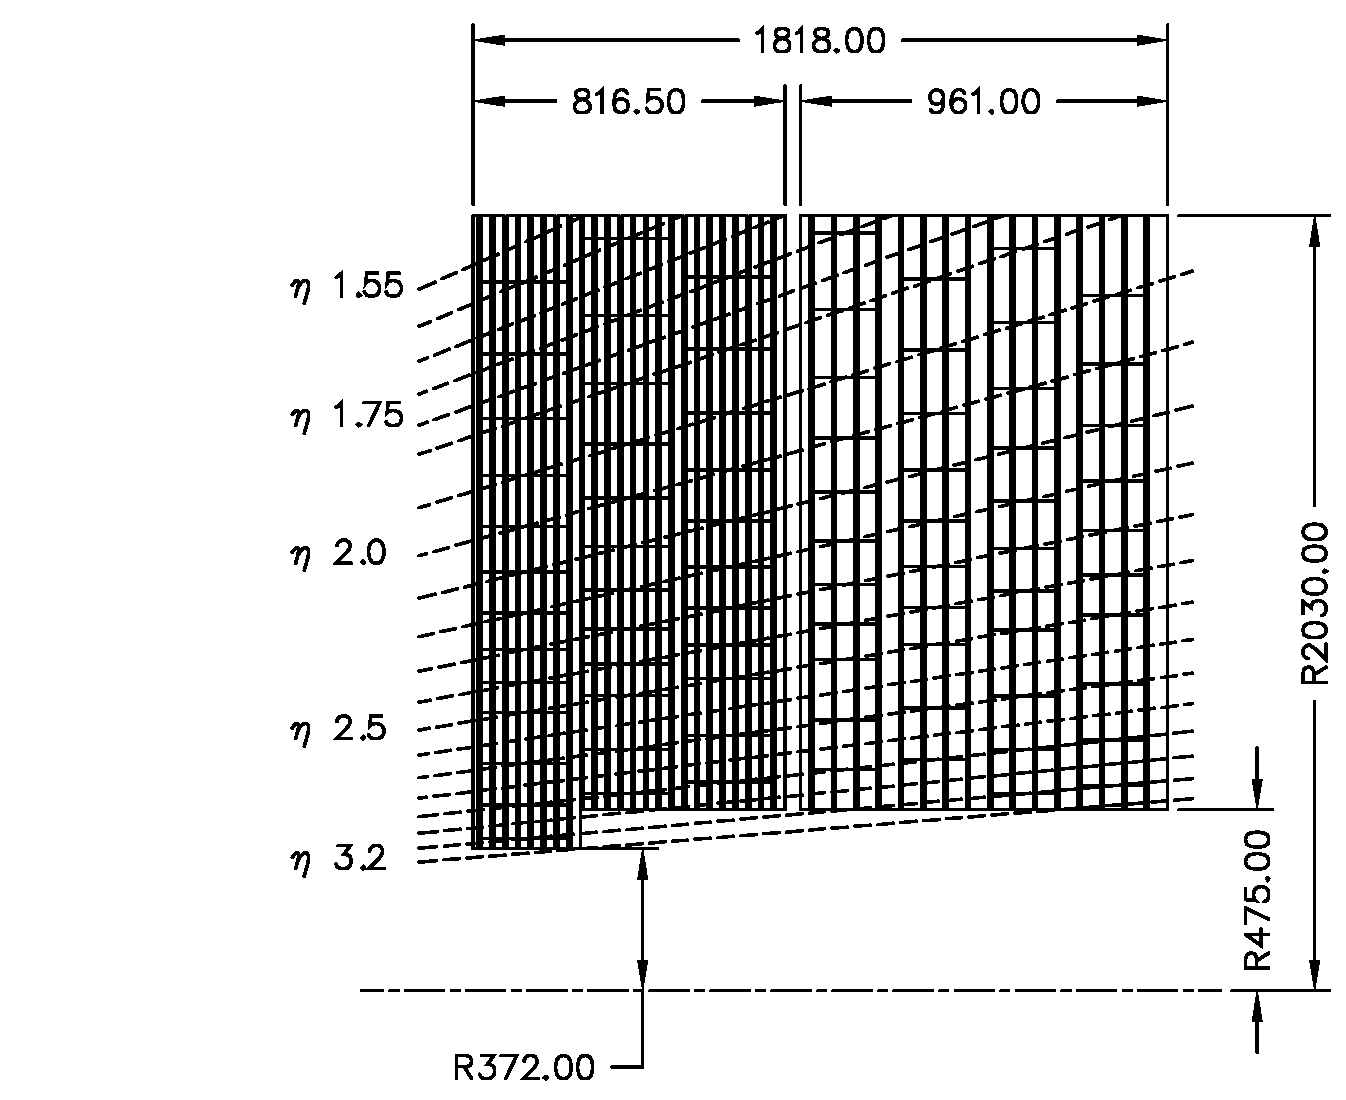
\includegraphics[width=.7\textwidth]{figures/atlas/hec.pdf}
\caption{ A schematic showing one quadrant of the 
HEC system in the $R$-$z$ plane. The dashed lines indicate
the pointing direction achieved by the segmentation of the 
readouts.  Dimensions are in mm.  }
\label{fig:atlas_hec}
\end{figure}


The HEC is designed to measure hadronic energy deposits in the 
end-cap regions from $1.5 < |\eta|< 3.2$. It uses 
copper plates as the sampling material with LAr gaps
for the active material. Two separate wheels are formed from
flat plates of copper alternating with LAr gaps further divided by electrodes for
collecting the ionization charge from the hadronic shower in the LAr.
The rear wheel is more coarse than the front wheel,
as can be seen in the schematic of \fig\ref{fig:atlas_hec}.
The electronics readout is segmented such that pointing information
can be obtained, as indicated by the dashed lines.
The maximum radial depth of the HEC is roughly $10~\lambda$.



\begin{figure}[ht] 
\centering
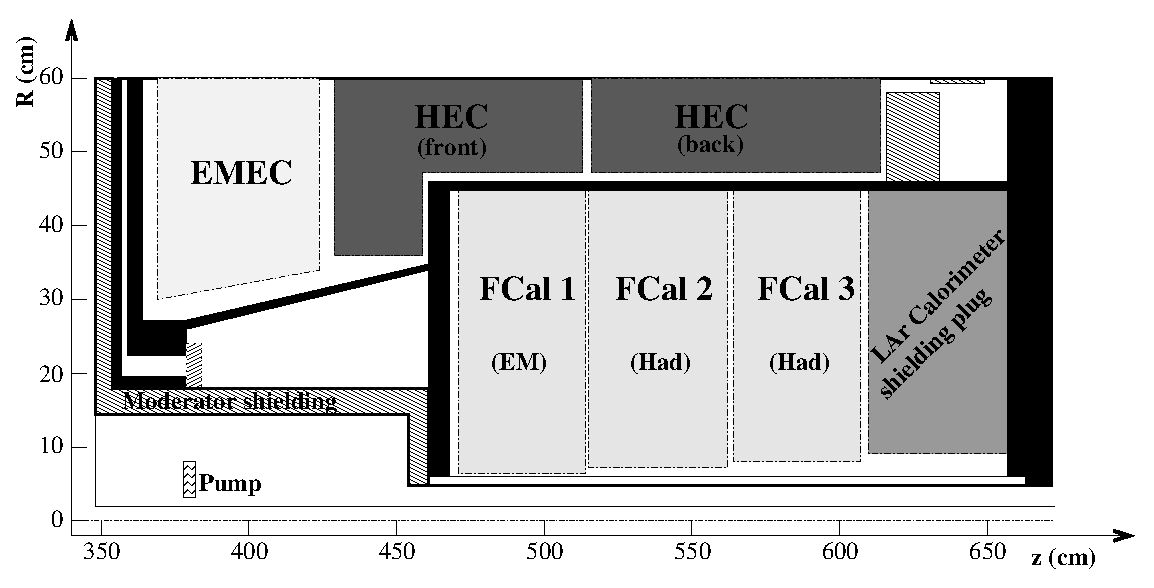
\includegraphics[width=.7\textwidth]{figures/atlas/fcal.eps}
\caption{ A schematic showing the end-cap of the ECAL,
the two HEC modules, and the three FCAL modules, as well
as additional shielding, in one
quadrant of the ATLAS detector as viewed 
in the $R$-$z$ plane.
The $R$-direction is shown with a larger scale than in the $Z$-direction.
}
\label{fig:atlas_fcal}
\end{figure}


The FCAL is in the region of the detector nearest to the beam-line, 
where the radiation flux is highest, covering the range
from $3.1 < |\eta| < 4.9$. It is split into three cylindrical modules,
oriented as in \fig\ref{fig:atlas_fcal}, with the first 
being designed for measuring electromagnetic deposits and the other
two for hadronic deposits.
Each FCAL module is constructed from copper plates with roughly ten thousand
uniformly spaced holes drilled in the direction parallel to the beam-line.
The holes are filled with rods serving as the primary sampling material, 
with a thin LAr gap surrounding the rods serving as the active material.
The first FCAL uses copper rods to optimize for electromagnetic deposits
while the second and third FCAL modules, use tungsten rods
to optimize for hadronic deposits.
The first FCAL has a radiation length of $27.6~\xzero$ and an 
interaction length of $2.66~\lambda$. Meanwhile, the interaction
length of the second and third modules is around $3.6~\lambda$.



Shielding? Resolution and response?




\section{Muon Spectrometer}
%do i want to talk about muon reconstruction?
%definitely mention muon resolution

\begin{figure}[ht]
\centering
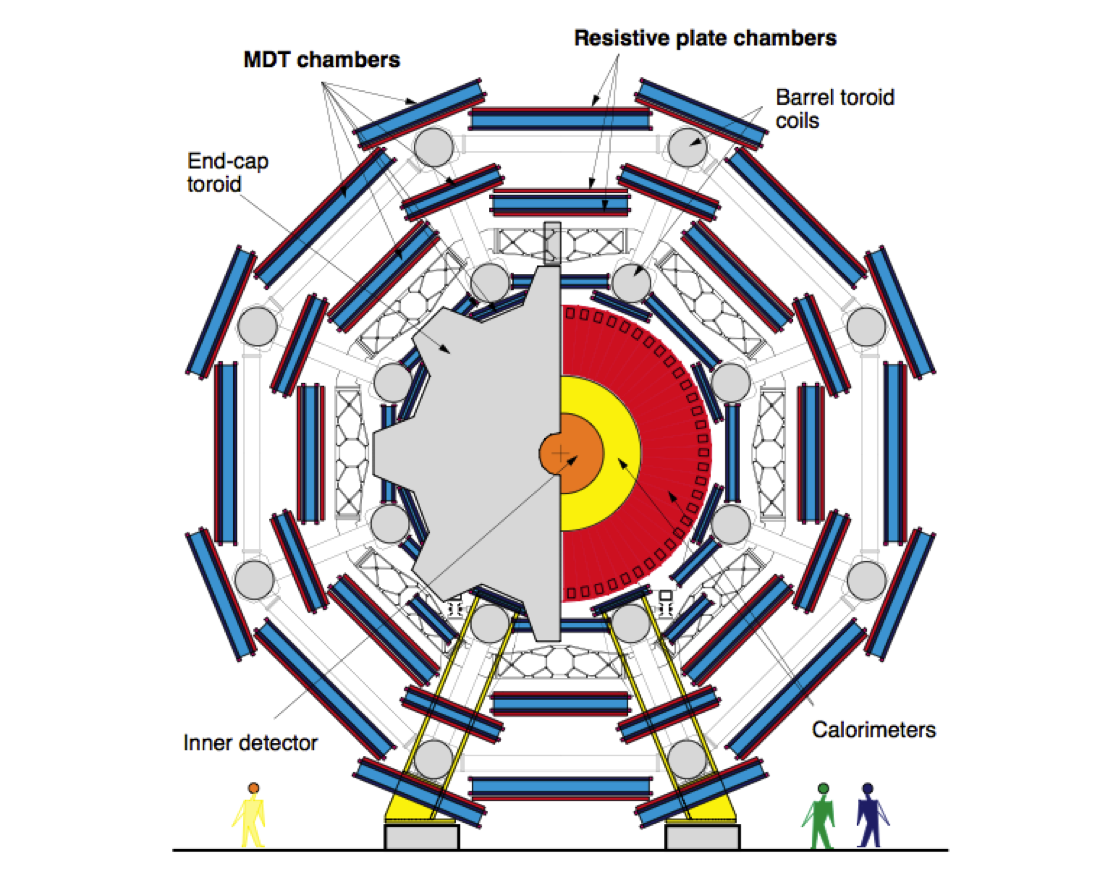
\includegraphics[width=.8\textwidth]{figures/atlas/ms_rphi}
\caption{A cross-section of the MS in the 
transverse ($r-\phi$) plane viewed from one end of the detector. 
The MDT chambers, RPCs, and
barrel and endcap toroids of the MS system are clearly labeled.
The barrel toroid coils extend in to and out of the page while only
half of the endcap toroid is shown to reveal the ID and calorimeter
systems.  The LHC beam pipe runs through the center.}
\label{fig:atlas_ms_rphi}
\end{figure}

\begin{figure}[ht]
\centering
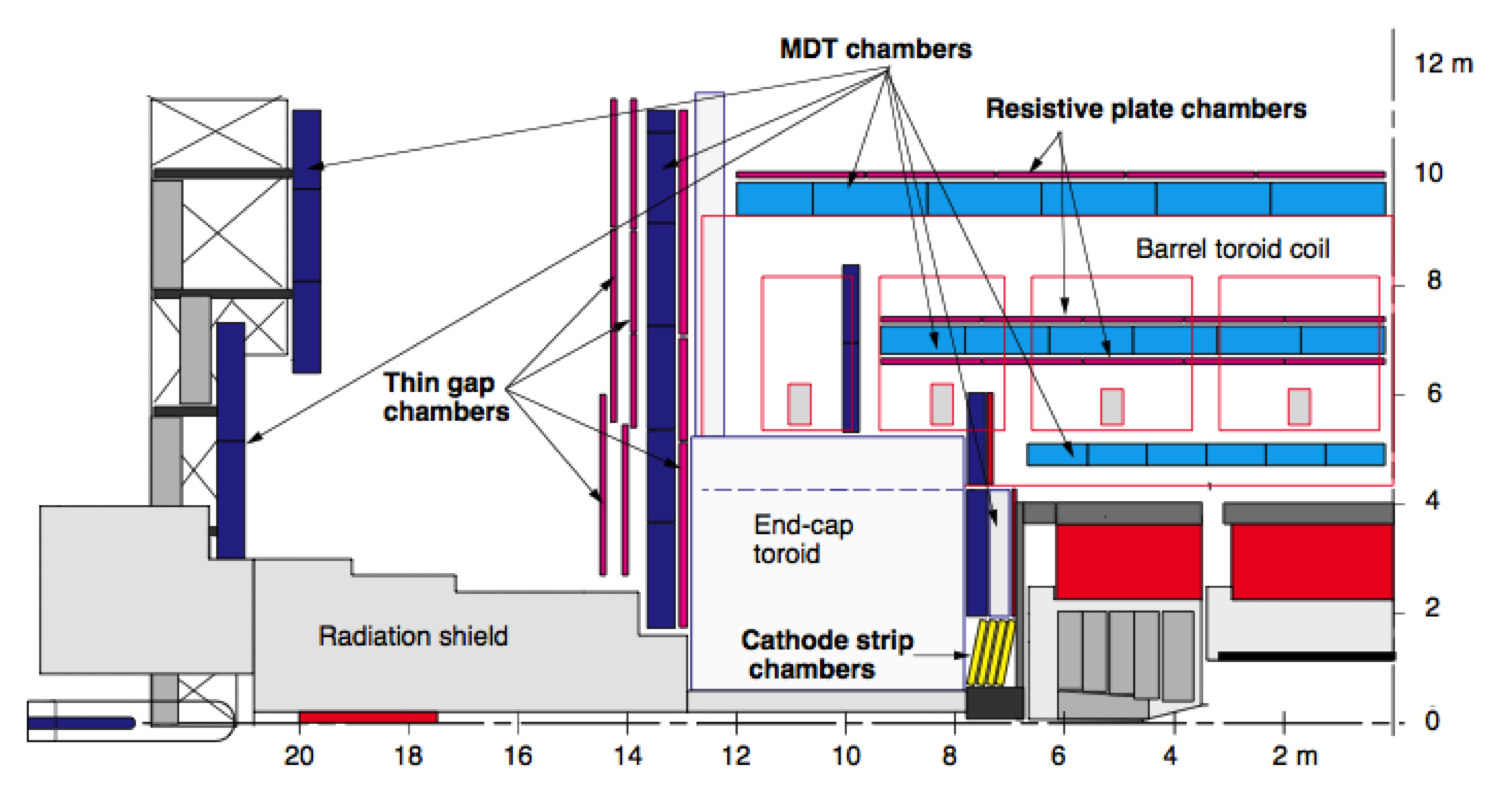
\includegraphics[width=.8\textwidth]{figures/atlas/ms_rz}
\caption{One quadrant of the MS as viewed in the $R-z$ plane. The
MDT chambers, RPCs, TGCs, CSCs are clearly indicated, as are the 
the endcap and barrel toroids. Support structues, shielding and the calorimeter
and ID systems are also drawn. The LHC beam pipe runs from left to right
along the bottom.}
\label{fig:atlas_ms_rz}
\end{figure}

The Muon Spectrometer (MS) is the largest component of the ATLAS
detector, being the component that determines its overall size. 
%The size is determined by the field strength and lever arm...
%maybe try to explain that... look in book that was taken...
It is designed to measure and identify muons as they
pass through the MS and leave the detector.
It surrounds the beam pipe, as well as the ID and calorimeter systems,
using a cylindrical geometry with a barrel and two endcaps. 
The MS is comprised of several different technologies:
Muon Drift Tubes (MDT) and Cathode Strip Chambers (CSC) are used as
precision tracking components for measurements of the muon 
trajectory, Resistive Plate Chambers (RPC) and 
Thin Gap Chambers (TGC) are used as triggering 
components with good timing resolution, 
and a toroidal magnet system is used for bending the muon trajectory 
in order to extract a momentum measurement.
A diagram of the MS in the transverse plane is shown in 
\fig\ref{fig:atlas_ms_rphi} where the MDT chambers and RPCs of the barrel
are clearly shown along with the barrel and endcap toroids.
Another view of the MS in \fig\ref{fig:atlas_ms_rz} is displayed in
one quadrant along the axial direction which
shows the barrel and endcap toroids, along with 
the MDT chambers in the barrel and endcap, the RPCs in the
barrel, and the CSCs and TGCs in the endcap.

%The physics requirements are...
\begin{figure}[ht]
\centering
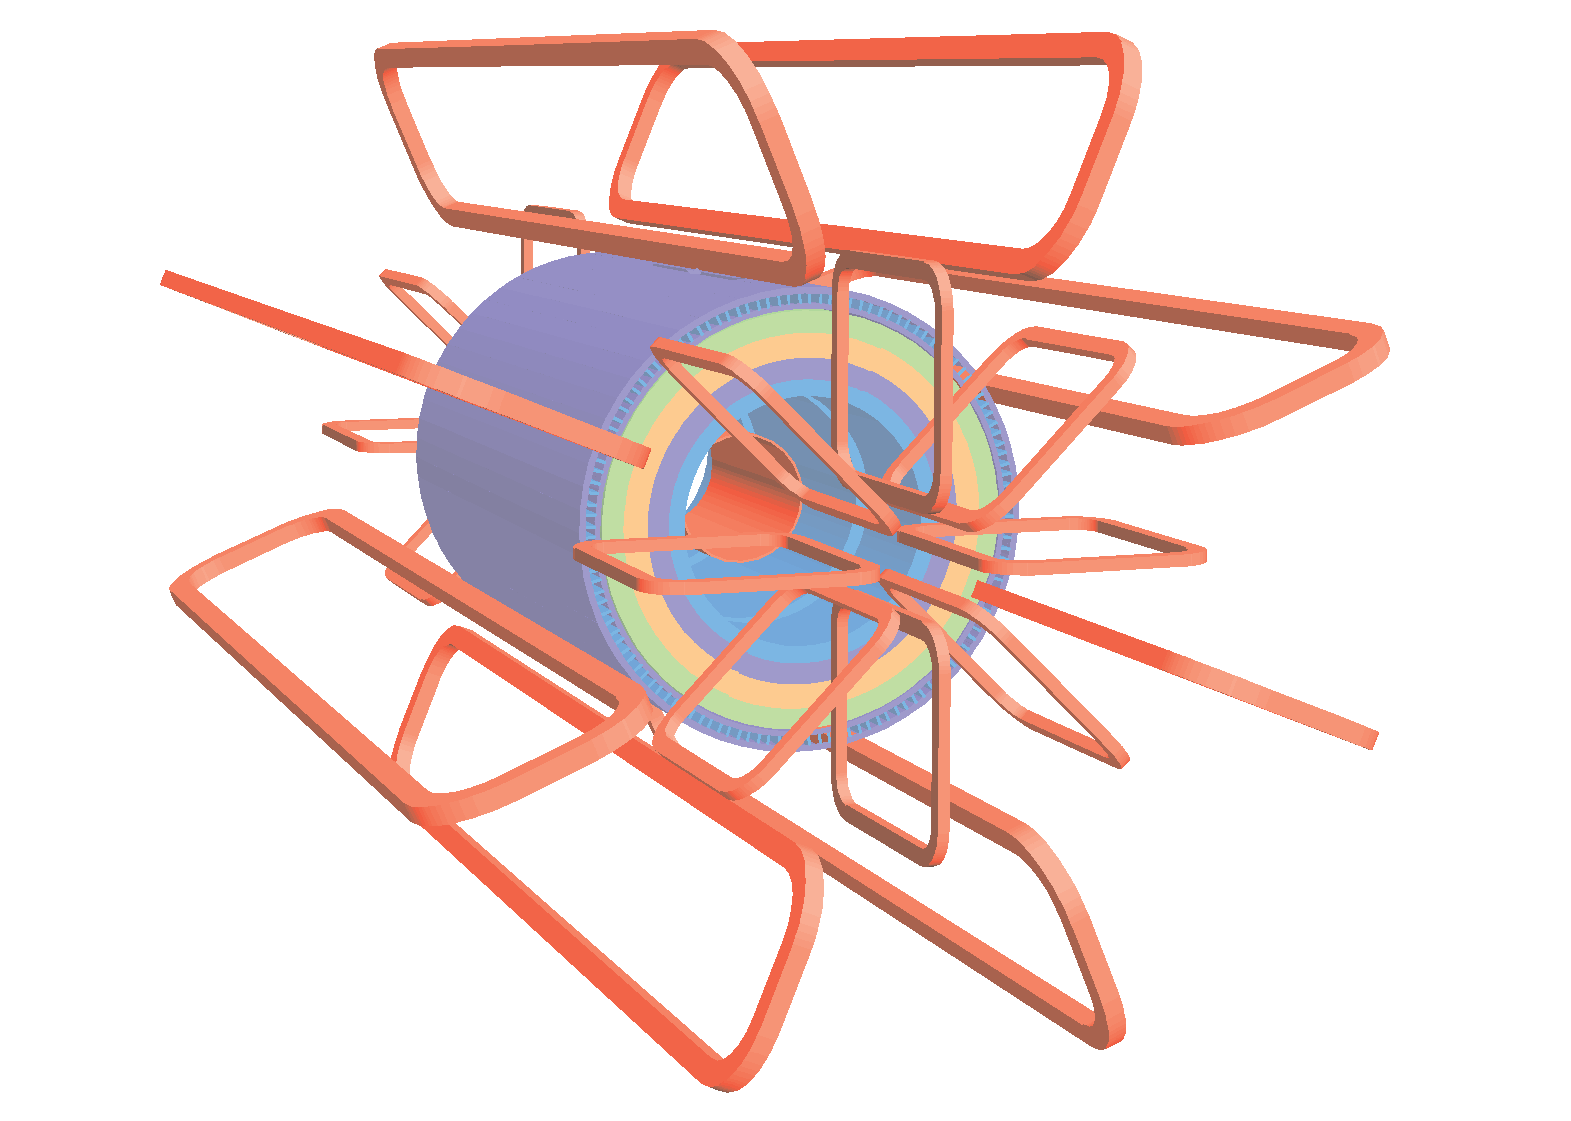
\includegraphics[width=.45\textwidth]{figures/atlas/magnet}
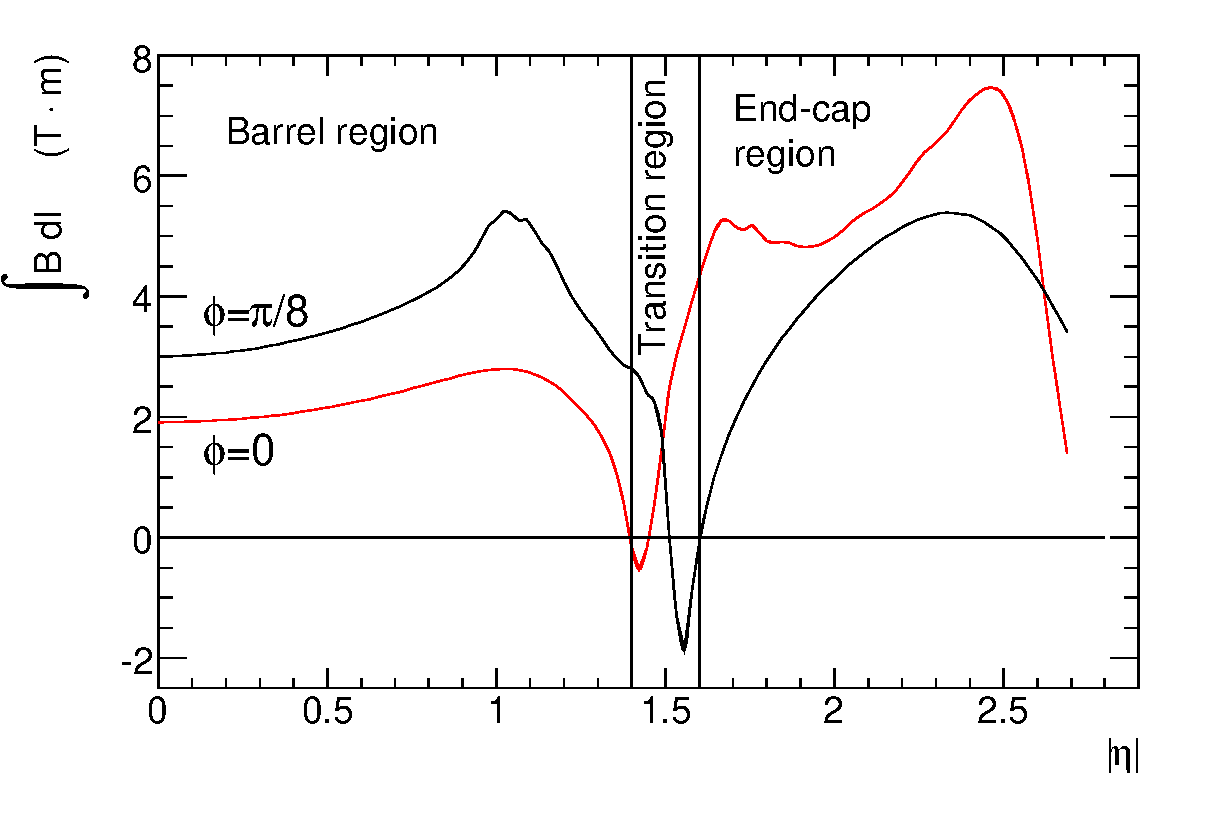
\includegraphics[width=.45\textwidth]{figures/atlas/toroid_magnet_field}
\caption{(Left) Diagram of MS toroid magnet geometry shown in red. The
tile calorimeter is also shown.
(Right) Predicted field strength of the MS magnet 
system as a function of $|\eta|$
for $\phi=0$ in red  and $\phi=\pi/8$ in black.}
\label{fig:atlas_toroid_magnet}
\end{figure}


The MS magnet system is composed of several large air-core toroids built
from superconducting coils which produce a magnetic field of 
roughly 0.5 Tesla in the barrel and 1 Tesla in the endcap. 
The geometry of the MS magnet system is shown 
on the left of \fig\ref{fig:atlas_toroid_magnet}. In the barrel, 
eight 25 m long toroidal 
coils inside stainlees-steel vacuum enclosures are placed uniformly in 
azimuth around the barrel. In the two endcaps, 
each endcap toroid is composed of 
eight square coils (rotated with respect to the barrel toroids)
separated by supporting wedges and then surrounded in a single 
cryostat.
The resulting field is non-uniform as can be seen on the right
of \fig\ref{fig:atlas_toroid_magnet}. 
The field strength in the transverse plane is roughly zero and so is referred
to as the non-bending plane, while the $\eta$ direction is referred to as the
bending plane.
To achieve adequate momentum resolution, the resulting field must be known
precisely.
The field is measured in all directions using sensors placed throughout
the MS and shown to usually agree with predictions within a few milli-Tesla.
The field is especially non-uniform in the region from 
$1.3 < |\eta| < 1.65$, referred to as the transition region, 
where the bending power of the field actually becomes zero
for certain values of $\eta$ and $\phi$.
This results in degraded momentum resolution and poor trigger efficiencies
in this region.


\begin{figure}[ht]
\centering
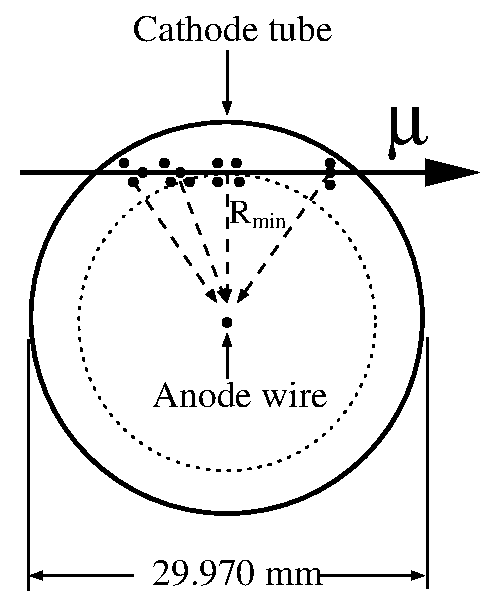
\includegraphics[width=.35\textwidth]{figures/atlas/ms_mdt_tube.eps}
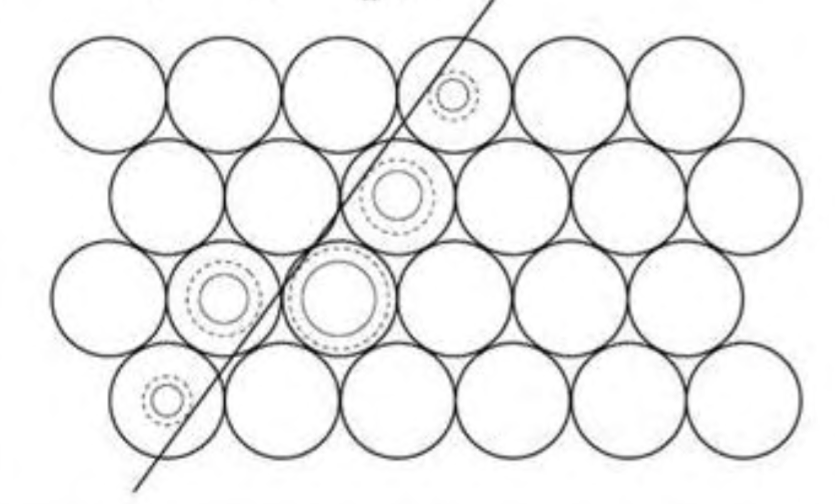
\includegraphics[width=.55\textwidth]{figures/atlas/ms_mdt_hits.png}
%ms_mdt_hits taken from http://arxiv.org/pdf/0810.3184.pdf
\caption{(Left) Cross-section of single MDT tube with muon track
passing through. Ionized electrons collect on the anode wire
due to the applied electric field. (Right) Muon track
reconstructed from array of MDT tubes.}
\label{fig:atlas_ms_mdt}
\end{figure}



\begin{figure}[ht]
\centering
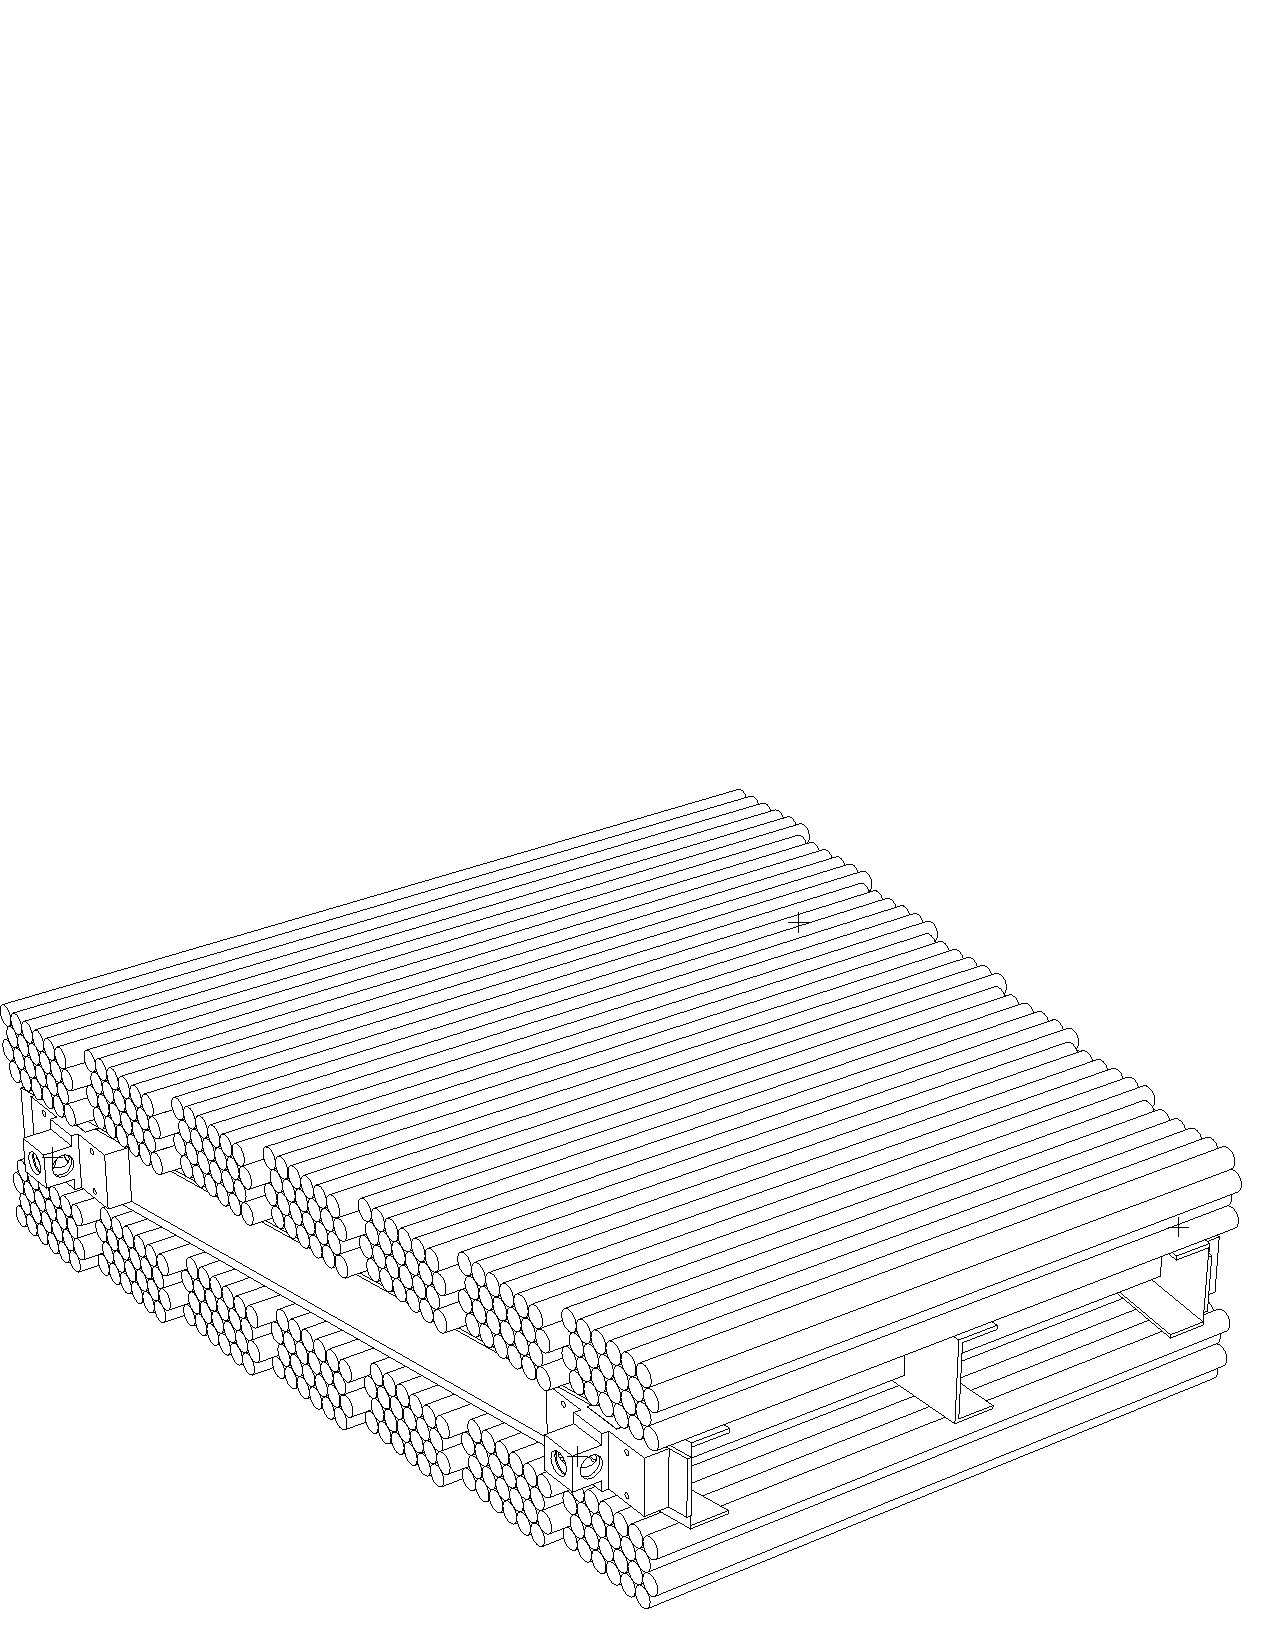
\includegraphics[width=.8\textwidth]{figures/atlas/ms_mdt_chamber.pdf}
%ms_mdt_hits taken from http://arxiv.org/pdf/0810.3184.pdf
\caption{Schematic of a single MDT chamber.}
\label{fig:atlas_ms_mdt_chamber}
\end{figure}

%figure taken from http://hedberg.web.cern.ch/hedberg/home/atlas/atlas.html

The precision tracking system has stringent requirements
on the precision of the muon trajectory measurement, 
which come from design goals on the resolution of the muon
transverse momentum mesaurement to be 
about 10\% at 1~\TeV.
Given the magentic field strength in the MS, a muon 
with this momentum is expected to have a sagitta
of about $500~\mu$m in the bending plane. 
According to \eqn\eqref{eq:sagitta},
this then translates into a precision requirement of 
no more than $50~\mu$m on the sagitta.
In order to achieve this, MDT chambers are used everywhere 
in the MS from $|\eta|<2.7$ except in the inner layer of the 
endcap from $2<|\eta|<2.7$
where the rates are too high. Here, CSCs are used instead. 
The MDT system is an arrangement of roughly 1000 MDT chambers composed
of aluminum drift tubes roughly 30 mm in diameter and a couple meters in length 
filled with a gas mixture
(Ar/CO2) and a high voltage wire (~3000 V)
running through the center. 
It was chosen as the main precision muon tracking system
because of its precision, simplicity, and reliability.
When a muon passes through an MDT
it ionizes the gas and electrons are collected at the wire.
The drift-time for the electron signal to collect on the wire
can be used to determine the radial distance away from the wire
at which the muon passed such as on the left of \fig\ref{fig:atlas_ms_mdt}. 
The cylindrical symmetry
of the tube is useful as the resolution is roughly flat, at around
$80~\mu$m in the bending plane, as a function
of the angle of incidence of the muon hitting the tube. 
It is not possible, however, to determine the direction
of the muon in the bending plane from just one tube.  For that reason, 
tubes are arranged together in multi-layers of 3-8 tubes such that 
the trajectory
can be reconstructed from matching the pattern of hits in multiple layers
to form track segments,
such as on the right of \fig\ref{fig:atlas_ms_mdt}.
A chamber is built from 2 multilayers separated by a spacer ranging from
6 mm to 300 mm wide depending on 
the chamber, as in \fig\ref{fig:atlas_ms_mdt_chamber}.
The precision per chamber is roughly $35~\mu$m.
The long length of the MDTs means that they cannot provide a  useful measurement
in the non-bending plane.
Chambers are arranged in three concentric shells in the barrel 
at $r = $5 m, 7.5 m, and 10 m as in \fig\ref{fig:atlas_ms_rphi} 
and in several rings in the endcap
at $|z| = $7.4 m, 10.8 m, 14 m, and 21.5 m as in \fig\ref{fig:atlas_ms_rz}.
In each shell or ring
the chambers are made to overlap in order to avoid gaps in azimuth.
Tracks  are then reconstructed using by interpolating between the 
track segments of the individual chambers.
Still, there are gaps, in particular around $|\eta|=0$ due to a hole for services
and due to the feet holding up the detector, seen in \fig\ref{fig:atlas_ms_rphi}.
An optical alignment system is used to monitor the MDT chambers %alignment between chambers?
for deformations. The tension of the wires can also be adjusted
to account for sag where needed. %technically only in barrel.
Despite having very good precision, the maximum drift time
can be as high as 700 ns, which is far too slow for LHC bunch identification.


\begin{figure}[ht]
\centering
\includegraphics[width=.7\textwidth]{figures/atlas/ms_csc_disk.eps}
\caption{Diagram showing the arrangement of the CSCs in the endcap.}
\label{fig:atlas_ms_csc_disk}
\end{figure}


The CSC are used in the region of the MS closest to the interaction
point where the crossing rate of tracks 
is greater than $150$ Hz/cm$^2$, 
too high for succesful operation of the MDT chambers.
The CSCs can handle up to 1000 Hz/cm$^2$
while maintaining adequate  precision in the bending plane.
A CSC is a multiwire proportional chamber
composed of planes of cathode strips sandwhiching 
a row of parallel anode wires and filled with a non-circulating gas (Ar/CO2)
in the gap.
The two planes of cathode strips are separated by 5mm
with the anode wires running directly between the two planes.
A signal is induced on the cathode strips due to an avalanche
of electrons from the ionizing muon collecting on the anode wire.
The two planes of cathode strips are segmented in orthogonal directions
providing measurements in both the bending and non-bending planes of the detector. 
A CSC is composed of four of these layers, each giving separate $\eta$ and
$\phi$ measurements.
The resolution in the bending plane is roughly 60 $\mu$m
while the coarser segmentation in the non-bending plane 
results in a  resoulution of  roughly 5 mm.
Two rings are formed from the chambers such that the anode wires
point radially such that there are no gaps in $\phi$, as
can be seen in \fig\ref{fig:atlas_ms_csc_disk}. The rings are positioned
at roughly $|z|=7.5$ m. The rectangular symmetry of the individual channels
results in a degradation of the resolution based on the angle of incidence.
This is resolved by titling the chambers slightly toward the interaction point.
Of use in the high occupancy environment, 
if multiple tracks are present in a CSC in a given event, 
the signal pulse height can be used to match the tracks.
The small separation between cathode strips results in a layer
results in a short electron drift time allowing for a good
timing resolution of about 7 ns per layer.

optical alignment? Resolution?
\begin{figure}[ht]
\centering
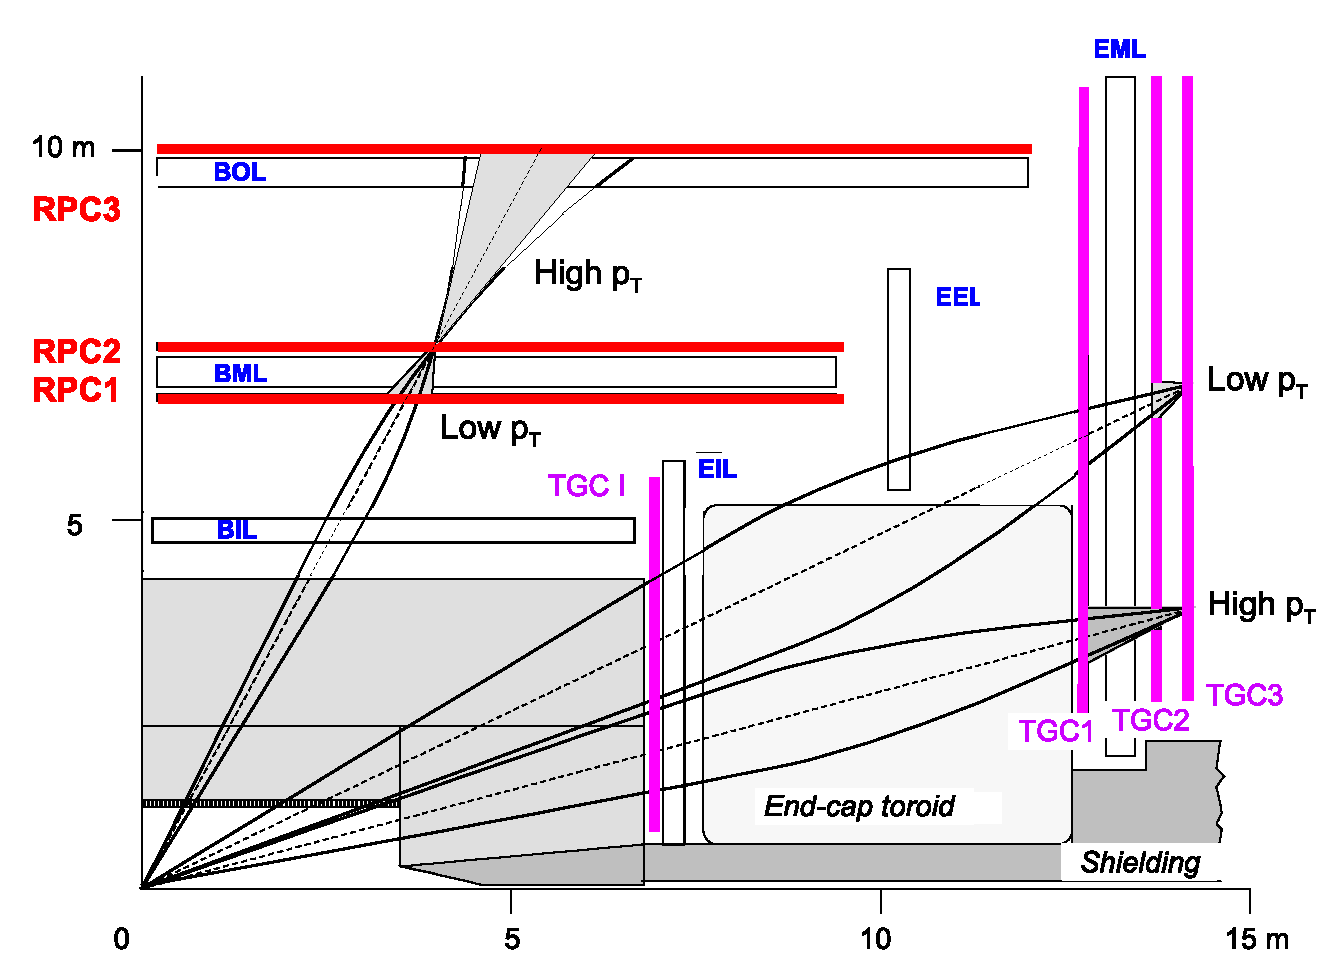
\includegraphics[width=.7\textwidth]{figures/atlas/ms_trigger_layout.eps}
\caption{Layout of the trigger components for one quadrant
in the $r-z$ plane. RPC and TGC chambers are cleary labeled. Possible
muon trajectories are seen for low and high \pt roads formed
by the trigger algorithm (see \sec\ref{sec:atlas_trigger}).}
\label{fig:atlas_ms_trigger_layout}
\end{figure}

The triggering system in the MS is designed to be able
to identify muons coming from individual bunch crossings of the LHC
and to discriminate them based on their position and \pt~in the region
$|\eta|<2.4$. This information
is then used to trigger on high \pt~muons, as 
described in \sec\ref{sec:atlas_trigger}.
The individual bunch crossings of the LHC are designed to 
be separated by only 25 ns, as described in \sec\ref{sec:lhc}.
Thus, the system must be able to resolve individual tracks 
with a time resolution of this size.
%(what exactly is the design req?).
To distinguish high \pt~muons from straight-track neutral particles 
or from curved-track low-momentum charged particles, the 
system must be able to measure the sagitta of the 
trajectory in the toroidal magnetic field, though not necessarily
with the same precision as in the precision tracking system.
Furthermore, to distinguish individual tracks, position measurements
must be performed in both the bending and non-bending planes.
The measurement in the non-bending plane is also used to complement
the measurements of the bending plane from the MDT chambers.
RPCs are used in the barrel region
from $|\eta|<1.05$ and TGCs in the endcap from $1.05 < |\eta|<2.4$.
The layout of the triggering system can be seen in the diagram
in \fig\ref{fig:atlas_ms_trigger_layout}. 
The RPCs are parallel electrode-plate detectors which use no wires.
A single RPC layer consists of 
resistive plates aligned in parallel and separated by 2 mm 
with a gas mixture (primarily $\textrm{C}_2\textrm{H}_2\textrm{F}_4$)
in the gap. An electric field of 4.9 kV/mm is applied between 
the plates which results in electron avalanches forming in the gas
along the track.
This gives a signal pulse time resolution of about 5 ns.
The pitch of the individual plates is 23 mm in $\eta$ and 35 mm in $\phi$.
A single RPC consists of two such layers.  Three concentric shells 
are formed from the RPCs around the beam line 
at about $r = $ 6.5 m, 7.5 m, and 10 m
as in \fig\ref{fig:atlas_ms_trigger_layout}.
The separation between the inner and outer layers 
allows for a discrimination of muons with $9 < \pt < 35~\GeV$
while the separation between the inner and middle layers allows for 
discrimination of low-\pt~muons with $6 < \pt < 9~\GeV$.
%Space resolution...maybe put sqrt(12) formula? look up to be sure.


The TGCs are multi-wire proporational chambers, similar to the CSCs.
In a single TGC layer, the cathodes are 
separated by 2.8 mm and the wire-to-wire pitch
is 1.8 mm.  A high voltage of 2900 V is applied to the anode wires
resulting in a quasi-saturated electron avalanche in the gas 
mixture (CO2/n-pentane) due to incident tracks.
The small wire-to-wire pitch and high voltage result in a good 
timing resolution for the signal pulse. The resulting
signal pulse resolution is dependent on the angle-of-incidence
of the incoming track, but still results in a signal width
within 25 ns for about 99\% of tracks.
TGC chambers are built from either two or three layers. 
The TGC chambers are then arranged in rings such that they overlap
in azimuth to eliminate gaps.
The TGC rings are arranged as in 
as in \fig\ref{fig:atlas_ms_trigger_layout}
with a ring of two-layer TGCs placed in front of the endcap MDT inner
layer at about $|z|=7$ m, 
a ring of three-layer TGCs placed in front of the endcap MDT
middle layer at around $|z|=13 $m, and two rings of 
two-layer TGCs placed just behind
the endcap MDT middle layer at around $|z|=14$ m.
%pt resolution and performance?



\section{Trigger}
\label{sec:atlas_trigger}

The very small design collision bunch spacing 
of 25 ns (40.08 MHz) at the LHC combined with the average digitized event size
of around 1 Megabyte means that to record every collision
would require a bandwidth of around 40 Terabytes per second, far surpassing
the capabilities of modern hard-disks. Clearly recording every collision
is untenable. Fortunately, the type of collisions of interest at the LHC 
(high \pt~leptons and jets, high \met) are sufficiently rare 
that most of these collisions can be filtered out. 
This is accomplished by using a so-called ``triggering'' system, 
that quickly analyzes course information about the collision
and only records those collisions deemed interesting.
This is accomplished in stages. The 40.08 MHz collisions are
first passed to a custom electronics Level-1 (L1) trigger, designed
to reduce the rate to below 75 kHz; it then is passed to the 
relatively simple software based Level-2 (L2) trigger, designed to reduce the rate
to no more than 3.5 kHz; finally, it is passed to the third stage,
called the Event Filter (EF), which uses a more complex software-based 
selection similar to the offline selection, reducing the 
rate to below 200 Hz. The L2 and EF triggers are referred to together
as the High-Level Trigger (HLT). This results in a much more reasonable 
bandwidth for writing the data of about 0.2 Gigabytes per second.
To achieve these goals requires careful design and also (sometimes difficult)
choices about what types of collisions to keep.  This is discussed in more
detail below. 

The L1 trigger system is designed to use reduced granularity information
from the calorimeter and muon systems and custom electronics
to make on-the-fly decisions about interesting physics objects.
The inner detector is not used at L1.
Information about muons is taken from the coarse muon track measurements of 
the RPC and TGC components of the MS
as described in \sec\ref{sec:atlas_ms}. This information is 
used to build coarse trajectories called roads. The width of the road
is used to make one of a few possible \pt~cuts on the 
trajectory in the range of roughly $6<\pt<35~\GeV$. 
Meanwhile, information from the 
calorimeters is limited to coarse trigger ``towers'' mostly of dimension
$0.1 \times 0.1$ in $\Delta\eta \times \Delta\phi$.
Look-up-tables are used to quickly identify the transverse energy 
and this is summed using several sliding window algorithms to identify 
high \pt~electrons and photons, hadronically decaying taus, jets, large \met,
or large \et. 
In both the L1 muon and calorimeter triggers, special care is taken
to account for object multiplicities and to not double count. 
One important challenge is that the 
calorimeter signals and muon time of flight are slow enough\footnote{One
of the rare instances where the speed of light can be considered slow!}
that the signals from multiple bunch crossings occur in the detector
simultaneously.  Thus, each signal must be carefully synchronized with 
the bunch crossing from which it came.  
This must also account for the latency of the trigger itself, which
is around 2 $\mu$s.  The information
from the L1 muon and calorimeter triggers are passed to the Central
Trigger Processor which makes a decision about whether or not to pass
the event to the L2 trigger.  It does this by testing 
a number of possible conditions (for example, is there at least one
muon with $\pt > 15 \GeV$?) and then taking the logical OR of all of
these conditions.

The L2 trigger takes as input so-called ``Regions-of-Interest'' (RoI)
which are provided by the L1 trigger (for example, a cluster of 
trigger towers or a muon road). By restricting to RoIs,
the L2 trigger need only consider about 1-2\% of the 
total event\footnote{There are some instances of the L2 trigger
using the full event, but this is used sparingly.}. 
The L2 trigger runs simplified reconstruction algorithms in the RoIs 
on a computer processing farm. 
Once again, a number of  (more detailed) conditions are tested
to investigate 
if an interesting physics object really is present in the RoI.
If so, those conditions which returned a positive result are 
passed to the EF.

The EF is also run on a processor farm, but runs reconstruction algorithms
which are very similar to thos run during offline reconstruction.
In many cases the EF will run on the full event. The conditions
that were satisfied in L1 and L2 determine which algorithms and conditions
are run in the EF.  The list of conditions tested at the EF (and 
how they are connected to the L1 and L2) is referred to as the trigger menu.
The trigger menu can have hundreds of items.
Given the finite bandwidth of the trigger, the trigger menu
must be carefully chosen as not all are created equal. Some 
trigger items can take up a lot of bandwidth, some not.
Some might be considered essential, some obscure.
To mitigate this problem, some trigger items might be ``pre-scaled'',
meaning they are only kept some random fraction of the time.
In the end, the trigger menu is an important statement about the physics
priorities of the collaboration.
If any of the trigger menu items are satisfied they are finally written to disk.

plots of trigger menu?

trigger performance?





more detailed information
about the RoI and 








trigger menu.
mention my triggers.






\section{LUCID?}
